% Options for packages loaded elsewhere
\PassOptionsToPackage{unicode}{hyperref}
\PassOptionsToPackage{hyphens}{url}
%
\documentclass[
]{book}
\usepackage{amsmath,amssymb}
\usepackage{lmodern}
\usepackage{iftex}
\ifPDFTeX
  \usepackage[T1]{fontenc}
  \usepackage[utf8]{inputenc}
  \usepackage{textcomp} % provide euro and other symbols
\else % if luatex or xetex
  \usepackage{unicode-math}
  \defaultfontfeatures{Scale=MatchLowercase}
  \defaultfontfeatures[\rmfamily]{Ligatures=TeX,Scale=1}
\fi
% Use upquote if available, for straight quotes in verbatim environments
\IfFileExists{upquote.sty}{\usepackage{upquote}}{}
\IfFileExists{microtype.sty}{% use microtype if available
  \usepackage[]{microtype}
  \UseMicrotypeSet[protrusion]{basicmath} % disable protrusion for tt fonts
}{}
\makeatletter
\@ifundefined{KOMAClassName}{% if non-KOMA class
  \IfFileExists{parskip.sty}{%
    \usepackage{parskip}
  }{% else
    \setlength{\parindent}{0pt}
    \setlength{\parskip}{6pt plus 2pt minus 1pt}}
}{% if KOMA class
  \KOMAoptions{parskip=half}}
\makeatother
\usepackage{xcolor}
\usepackage{longtable,booktabs,array}
\usepackage{calc} % for calculating minipage widths
% Correct order of tables after \paragraph or \subparagraph
\usepackage{etoolbox}
\makeatletter
\patchcmd\longtable{\par}{\if@noskipsec\mbox{}\fi\par}{}{}
\makeatother
% Allow footnotes in longtable head/foot
\IfFileExists{footnotehyper.sty}{\usepackage{footnotehyper}}{\usepackage{footnote}}
\makesavenoteenv{longtable}
\usepackage{graphicx}
\makeatletter
\def\maxwidth{\ifdim\Gin@nat@width>\linewidth\linewidth\else\Gin@nat@width\fi}
\def\maxheight{\ifdim\Gin@nat@height>\textheight\textheight\else\Gin@nat@height\fi}
\makeatother
% Scale images if necessary, so that they will not overflow the page
% margins by default, and it is still possible to overwrite the defaults
% using explicit options in \includegraphics[width, height, ...]{}
\setkeys{Gin}{width=\maxwidth,height=\maxheight,keepaspectratio}
% Set default figure placement to htbp
\makeatletter
\def\fps@figure{htbp}
\makeatother
\setlength{\emergencystretch}{3em} % prevent overfull lines
\providecommand{\tightlist}{%
  \setlength{\itemsep}{0pt}\setlength{\parskip}{0pt}}
\setcounter{secnumdepth}{5}
\usepackage{booktabs}
\usepackage{amsthm}
\makeatletter
\def\thm@space@setup{%
  \thm@preskip=8pt plus 2pt minus 4pt
  \thm@postskip=\thm@preskip
}
\makeatother
\ifLuaTeX
  \usepackage{selnolig}  % disable illegal ligatures
\fi
\usepackage[]{natbib}
\bibliographystyle{apalike}
\IfFileExists{bookmark.sty}{\usepackage{bookmark}}{\usepackage{hyperref}}
\IfFileExists{xurl.sty}{\usepackage{xurl}}{} % add URL line breaks if available
\urlstyle{same} % disable monospaced font for URLs
\hypersetup{
  pdftitle={BOLD Room Instructions},
  hidelinks,
  pdfcreator={LaTeX via pandoc}}

\title{BOLD Room Instructions}
\author{}
\date{\vspace{-2.5em}}

\begin{document}
\maketitle

{
\setcounter{tocdepth}{1}
\tableofcontents
}
\hypertarget{introduction}{%
\chapter{Introduction}\label{introduction}}

This guide is designed to provide detailed instructions on how to use the BOLD room for video recordings of lecture material and tutorial videos. The guide contains three main sets of instructions:

\begin{itemize}
\tightlist
\item
  Setting up recording of lecture videos
\item
  Editing videos using Final Cut
\item
  Creating tutorial videos using the Wacom tablet
\end{itemize}

If you experience any issues using the equipment, please let us know at maths-stats-analyticsmsc-management@glasgow.ac.uk.

\hypertarget{book-a-time-slot}{%
\section{Book a time slot}\label{book-a-time-slot}}

Prior to your recording, you should ensure you have booked a time slot to use the BOLD room. When booking your time slot, be sure to consider setup time and any editing time of your video when planning how much time to book.

You can book a timeslot using the BOLD room calendar on the Maths \& Stats sharepoint page \href{https://gla.sharepoint.com/sites/school-maths-stats/Lists/BOLD\%20Room/calendar.aspx}{here}.

\hypertarget{accessing-the-bold-room}{%
\section{Accessing the BOLD room}\label{accessing-the-bold-room}}

In order to access the BOLD room, you will require SALTO access with your staff card. You will have to request access to the room from IT in order for your card to work.

\hypertarget{initial-room-setup}{%
\section{Initial room setup}\label{initial-room-setup}}

\begin{itemize}
\item
  The BOLD room can get rather cold in the winter months and the air conditioning does not switch on automatically. You may want to head down an hour or two prior to recording to switch this on.
\item
  Switch on the LED lights for the no entry sign at the door to notify people not to access as recording is taking place. The switch for these is behind the door as you enter.
\end{itemize}

\begin{figure}

{\centering 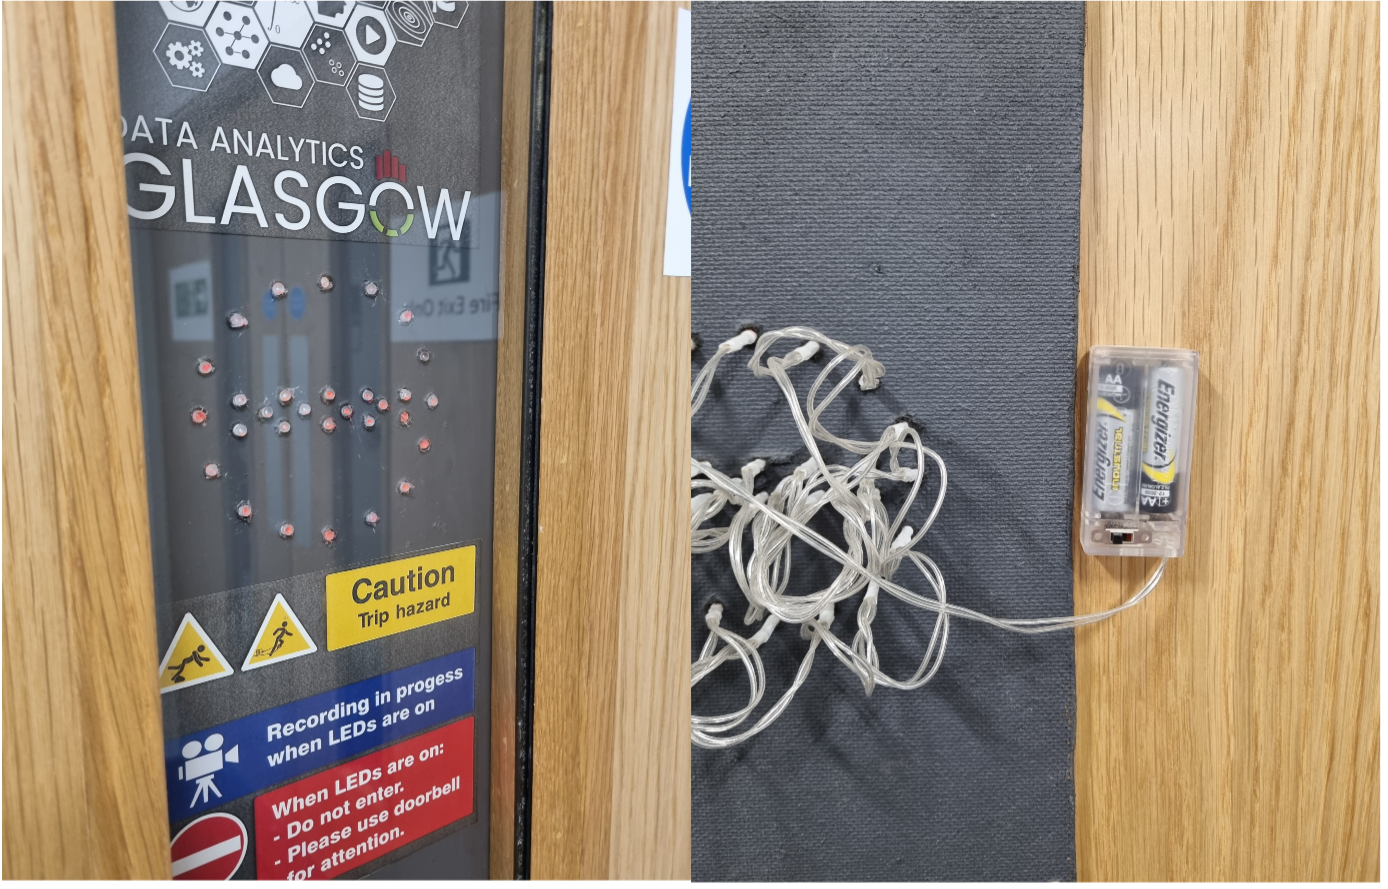
\includegraphics[width=1\linewidth]{Door_entrance} 

}

\caption{No-entry LED lights on door}\label{fig:door}
\end{figure}

\begin{itemize}
\tightlist
\item
  There is also a doorbell if someone needs to get your attention. The doorbell is set on silent but will glow to notify you that someone is at the door. The doorbell is located beside the HDMI matrix switch.
\end{itemize}

\begin{figure}

{\centering 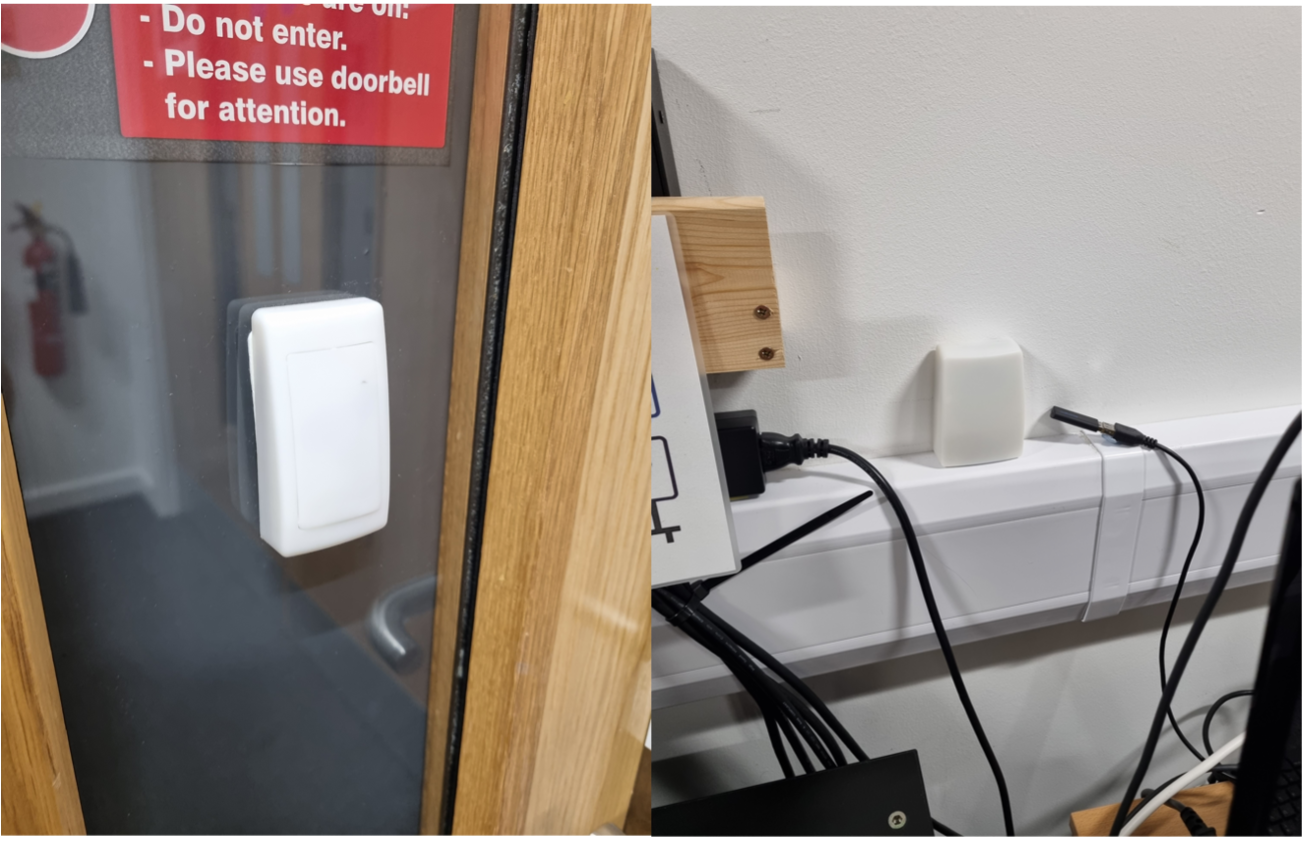
\includegraphics[width=1\linewidth]{Door_buzzer} 

}

\caption{Doorbell buzzer and location in BOLD room}\label{fig:buzzer}
\end{figure}

\hypertarget{intro}{%
\chapter{Video lecture recording in the BOLD room}\label{intro}}

These instructions provide information on how to record a video lecture recording, with the option to use the light board and incorporate slides.

\hypertarget{setting-up-for-recording}{%
\section{Setting up for recording}\label{setting-up-for-recording}}

\begin{itemize}
\tightlist
\item
  Switch on the HDMI matrix box. This will be used to select the desired displays from the monitors within the room. All monitors are labelled from A to D with an indication as to what output is being shown. There is also a remote control which can change outputs should you wish to use this when recording.
\end{itemize}

\begin{figure}

{\centering 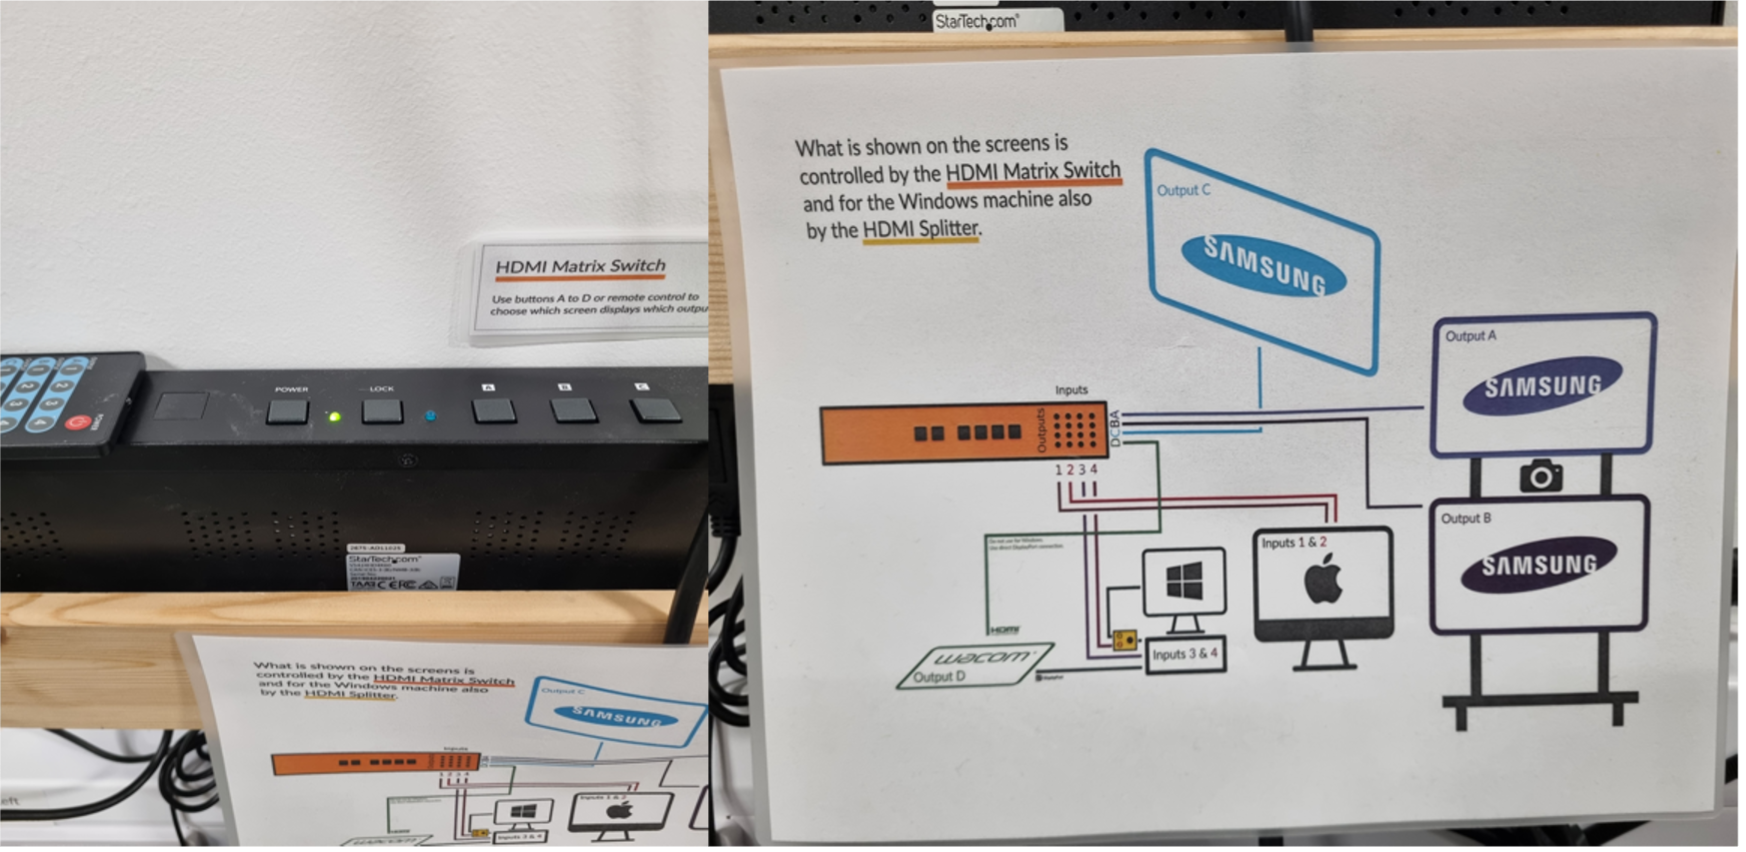
\includegraphics[width=1\linewidth]{HDMI_matrix} 

}

\caption{HDMI Matrix with instructions on channel connections}\label{fig:matrix}
\end{figure}

\begin{itemize}
\tightlist
\item
  Pull down the black curtain if you are recording. A yellow pulley is adjacent to the left-side wall which will lower the curtain.
\end{itemize}

\begin{figure}

{\centering 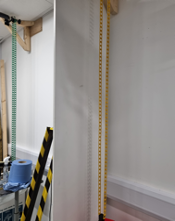
\includegraphics[width=0.6\linewidth]{Pulley} 

}

\caption{Pulley for curtain}\label{fig:curtain}
\end{figure}

\begin{itemize}
\tightlist
\item
  Switch on all of the lights here for recording. The switches for these are marked at the sockets around the room and shown below. Switch on the lightboard lights also if you intend to use this. The main room lights can be switched off (and will do automatically within 10 minutes as they are on a timer). Some of the lights are movable and feel free to adjust these as you wish for your recording.
\end{itemize}

\begin{figure}

{\centering 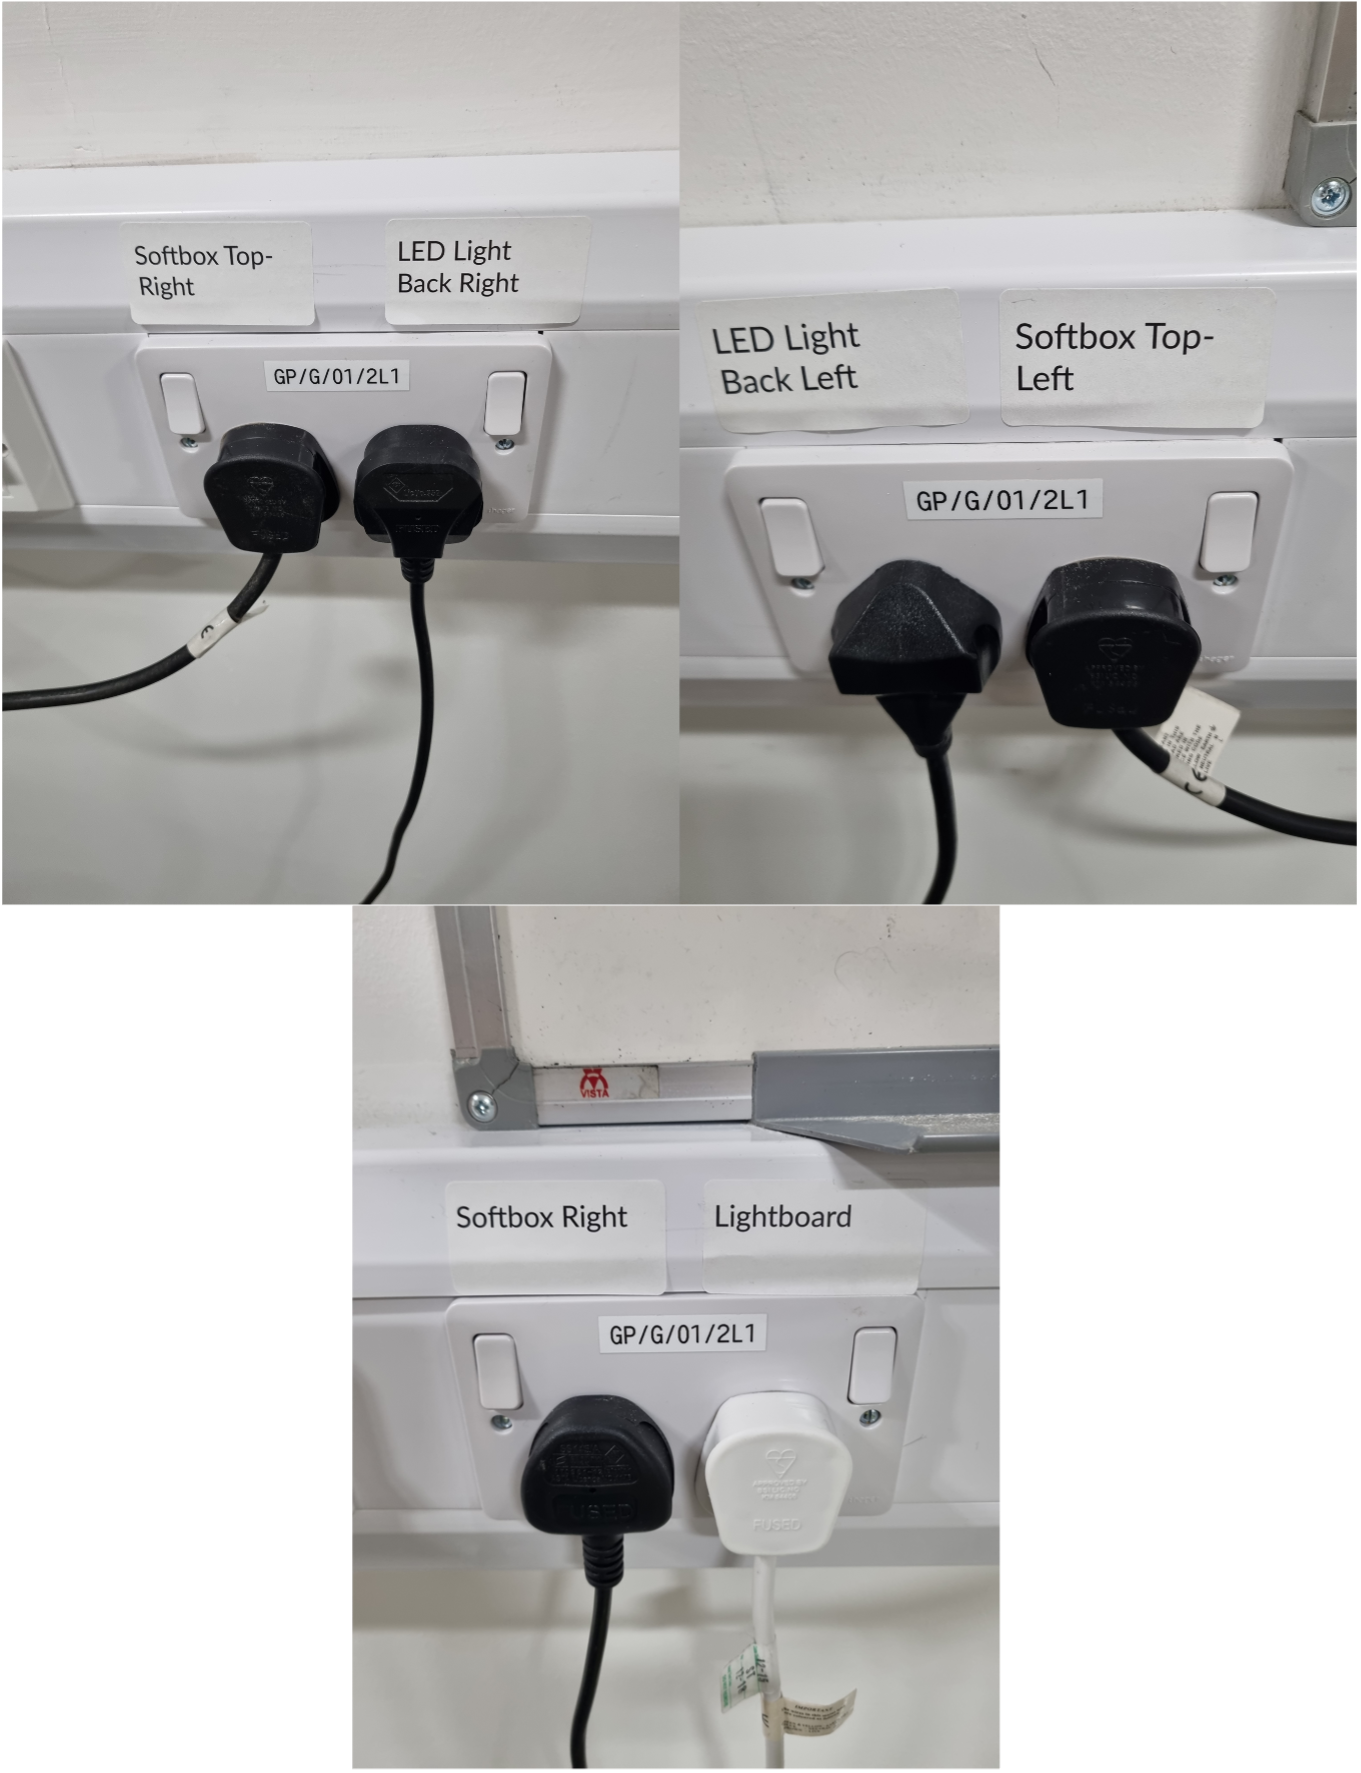
\includegraphics[width=1\linewidth]{Light_switches} 

}

\caption{Sockets for light switches to be used for recording}\label{fig:lightswitch}
\end{figure}

\hypertarget{preparing-the-recording-equipment}{%
\section{Preparing the recording equipment}\label{preparing-the-recording-equipment}}

\begin{itemize}
\item
  Switch on the Mac (ensure mouse and keyboard are also switched on). Log in using the BOLD account (password -- glasgow).
\item
  Switch on the camera for recording. Ensure the SD card is inserted prior to recording. The SD card can be accessed at the bottom of the camera.
\end{itemize}

\begin{figure}

{\centering 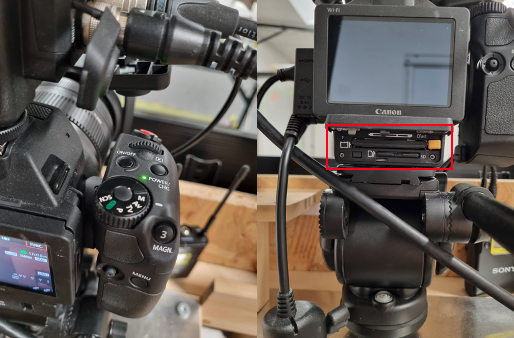
\includegraphics[width=1\linewidth]{Camera} 

}

\caption{Camera setup for recording}\label{fig:camera}
\end{figure}

\begin{itemize}
\tightlist
\item
  Ensure there is enough space on the SD card before you begin to record. You can check this by inserting the SD card into the D-link port behind the Mac.
\end{itemize}

\begin{figure}

{\centering 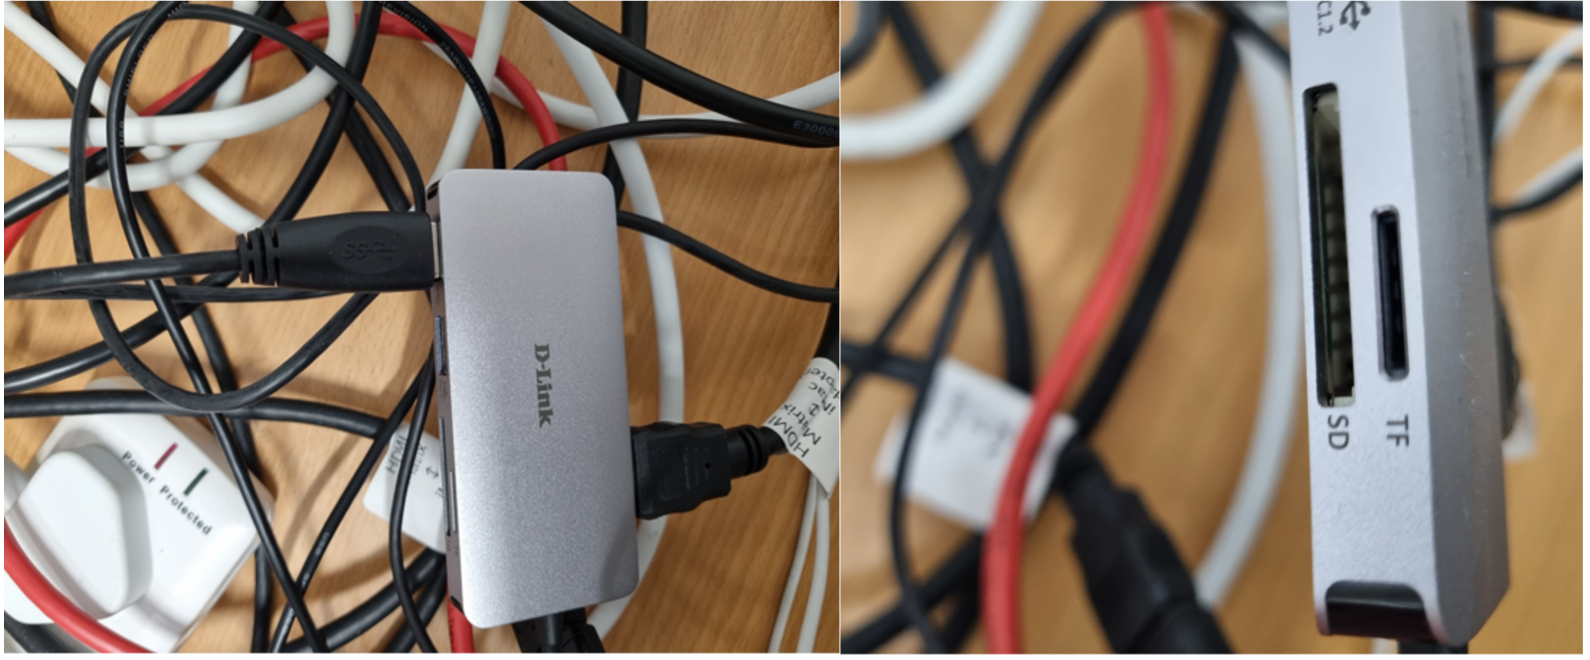
\includegraphics[width=1\linewidth]{Port} 

}

\caption{D-link port to connect SD card}\label{fig:port}
\end{figure}

\begin{itemize}
\tightlist
\item
  Switch on microphone pack. When wearing the pack, it is best to clip this on your side facing up, hiding the cable inside your top and attaching the mic to your collar. Also switch on the remote pack beside the camera. You can test that this is working by looking at the display and seeing the volume going up and down on the camera.
\end{itemize}

\begin{figure}

{\centering 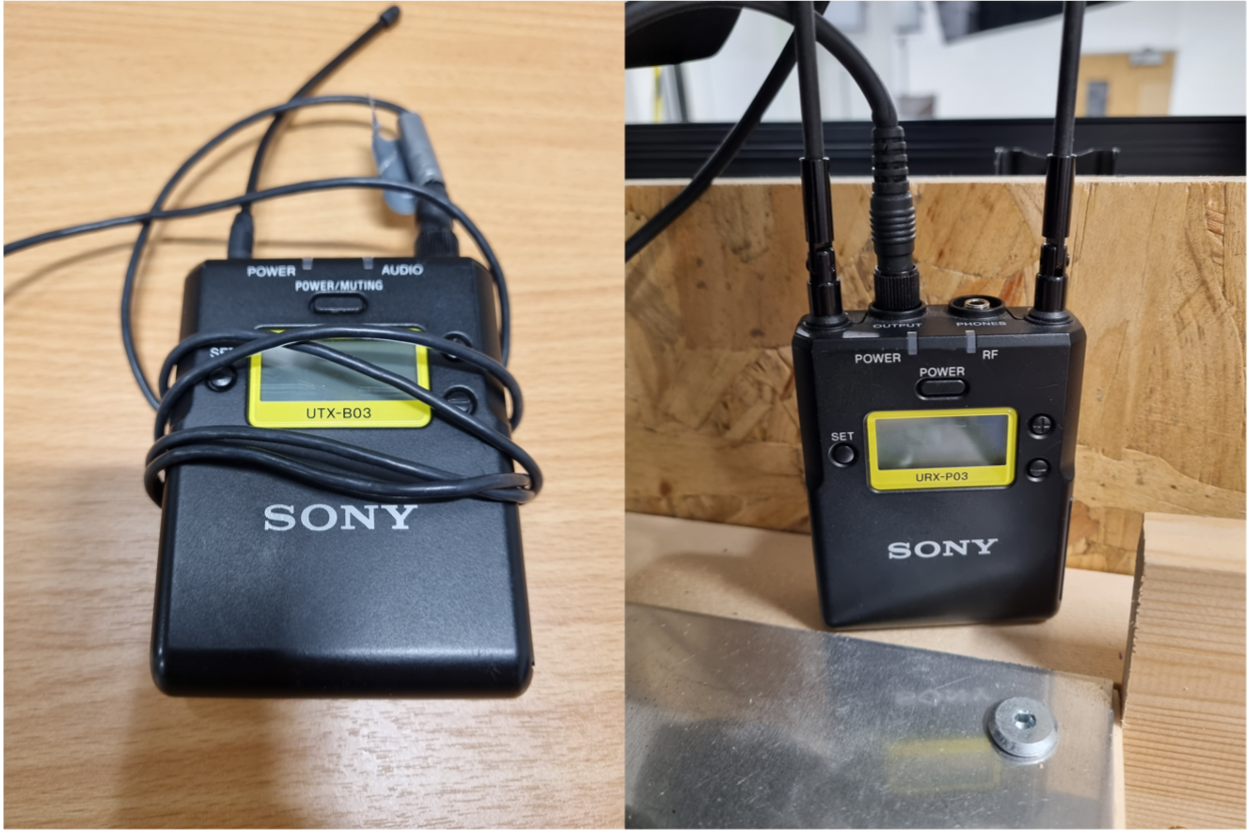
\includegraphics[width=1\linewidth]{Microphone} 

}

\caption{Microphone pack for recording with camera pack}\label{fig:microphone}
\end{figure}

\begin{itemize}
\tightlist
\item
  If neither pack is switching on, replace the batteries for these using the rechargeable batteries near the Mac. Be sure to charge any flat batteries. There are spare charged batteries in the cabinet in the right corner behind the Mac.
\end{itemize}

\begin{figure}

{\centering 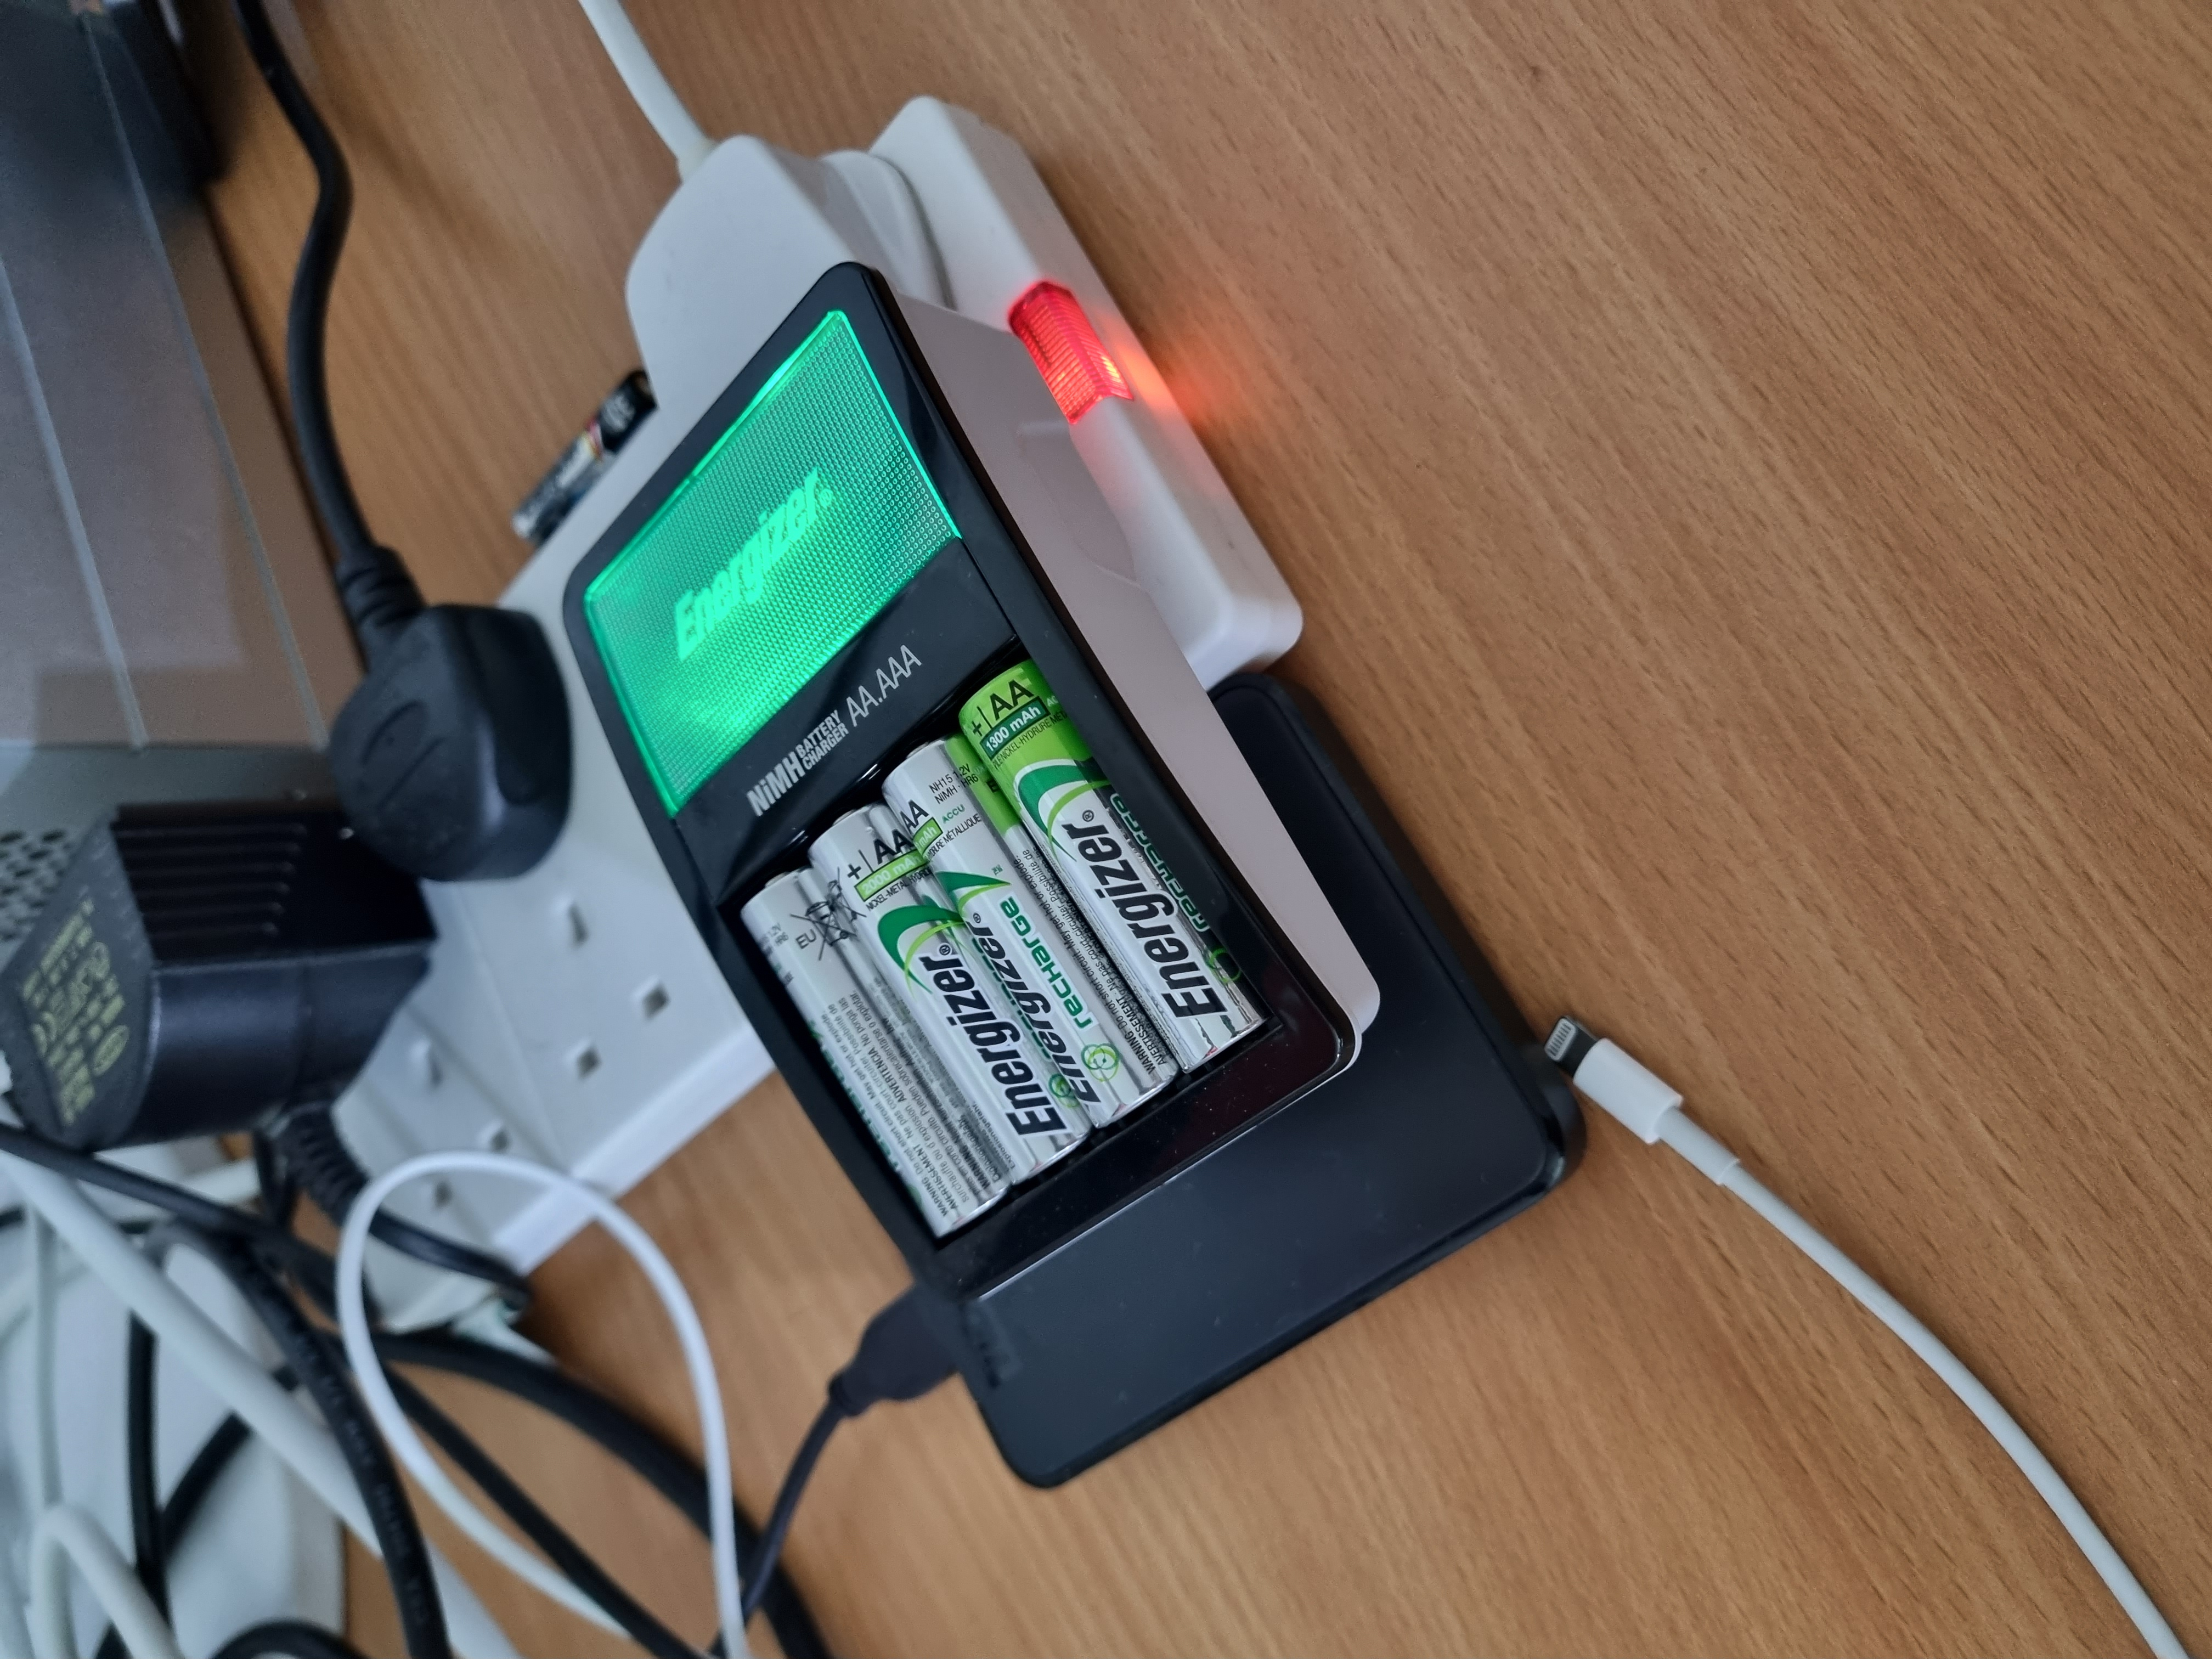
\includegraphics[width=0.6\linewidth]{Charger} 

}

\caption{Battery charger}\label{fig:charger}
\end{figure}

\begin{itemize}
\tightlist
\item
  Switch on the monitors. There is one Samsung remote which can be used to switch on all of the displays. Keep the remote close to the front of the display when switching on so this is picked up by the receiver.
\end{itemize}

\hypertarget{setting-up-the-mac-for-screen-capture-recording}{%
\section{Setting up the Mac for screen capture recording}\label{setting-up-the-mac-for-screen-capture-recording}}

\textbf{NB - if you are recording without slides or are using only the light board, skip this step for your recording}

\begin{itemize}
\item
  When you are recording with interacting slides or programming output (e.g.~R), you will record two videos

  \begin{itemize}
  \tightlist
  \item
    One from the camera with yourself and the light board
  \item
    One with a screen recording of the slides/programming output
  \end{itemize}
\item
  The camera output will be recorded on the SD card with the screen capture saved locally. If you are just recording yourself with no slides or using the whiteboard, you can skip the following steps and record directly off the camera.
\item
  To set up the second recording with the screen capture, first prepare your slides you wish to use onto one of the HDMI displays which you can select from the HDMI matrix. It is best to use one of the monitors in front of the camera for your slides. Drag the slides to the display you wish to use.
\item
  • With your slides, ensure these have a black background to prevent any issues with contrast in the recording. As a general guide, it is best to use slides in the style of the ODL slide template. An example set of slides is available on the desktop of the BOLD account.
\item
  Open the screen capture recording app which you can find in the dock as shown below
\end{itemize}

\begin{figure}

{\centering 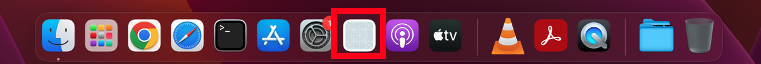
\includegraphics[width=1\linewidth]{App} 

}

\caption{App for screen capture}\label{fig:app}
\end{figure}

\begin{itemize}
\tightlist
\item
  Once opened, you will see a dialogue box open in your active window stating ``Record from the screen showing the other dialog?'' as shown below. You will then see an additional dialogue open on one of the other open screens reading ``This screen will be recorded''. If the screen you wish to record does not show the second dialogue box, press ``Swap'' on the first dialogue box which will switch screen recording to the other screen. Select ``Record'' once the second dialogue box is on the screen you wish to record.
\end{itemize}

\begin{figure}

{\centering 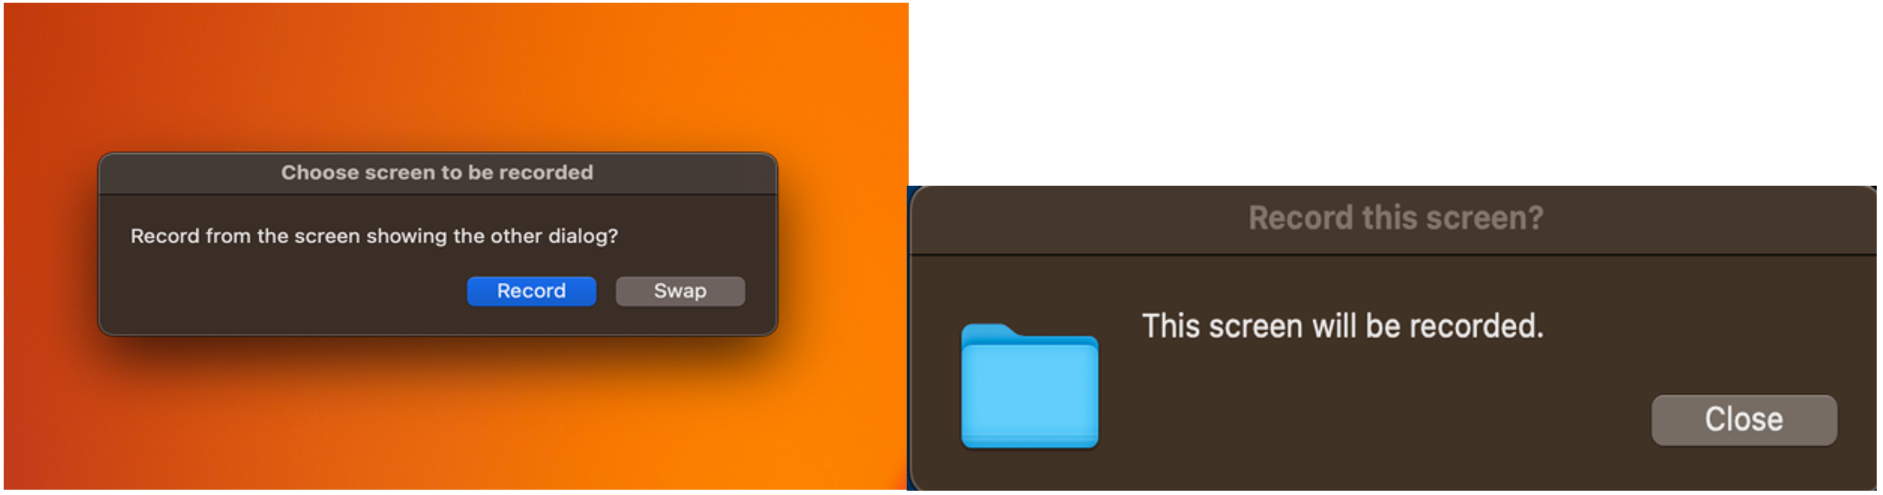
\includegraphics[width=1\linewidth]{Screen_capture} 

}

\caption{Commands for selecting screen to capture}\label{fig:screencapture}
\end{figure}

\begin{itemize}
\item
  You will then be asked to specify a location to save your screen capture. Set the folder to your own specified folder. \textbf{Ensure you keep the .mp4 file type in the name, else the video will not record!}
\item
  Another dialogue box should appear which will ask you ``Stop video recording?''. Leave this for now while you are recording your video.
\end{itemize}

\begin{figure}

{\centering 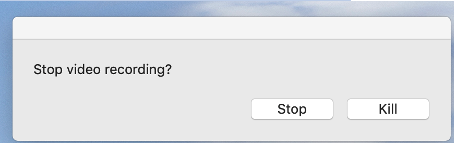
\includegraphics[width=1\linewidth]{Record_Stop} 

}

\caption{Stop recording action window}\label{fig:stoprecorde}
\end{figure}

\begin{itemize}
\item
  Press the record button (red button) on the camera to start recording from the camera. You should see a red light appear on the camera.
\item
  An additional window will open called ``Gstreamer video output'' Place this on an additional screen (usually on one of the monitors in front of the camera). This display allows you to see yourself with the screen recording of the slides/output so you can position yourself correctly throughout the recording.
\end{itemize}

\begin{figure}

{\centering \includegraphics[width=0.8\linewidth]{GStreamer} 

}

\caption{GStreamer output}\label{fig:gstreamer}
\end{figure}

\begin{itemize}
\item
  Use the clicker to change slides through your recording (be sure to make sure this window is selected first).
\item
  Once you have completed your recording, stop recording on the camera and then press ``Stop'' on the dialogue box on the Mac. Do \textbf{NOT} press ``Kill'' as this will terminate the process and the recording will not be saved!
\item
  You will now see your screen capture recording saved as an mp4 file in your specified location.
\item
  To import the camera capture, switch off the camera and remove the SD card from the port. Insert the SD card into the D-link port at the back of the Mac. You will be able to find your recording in the Canon drive in the Locations tab in Finder. The files should be chronologically ordered, so scroll to the bottom to find your recording.
\end{itemize}

\begin{figure}

{\centering 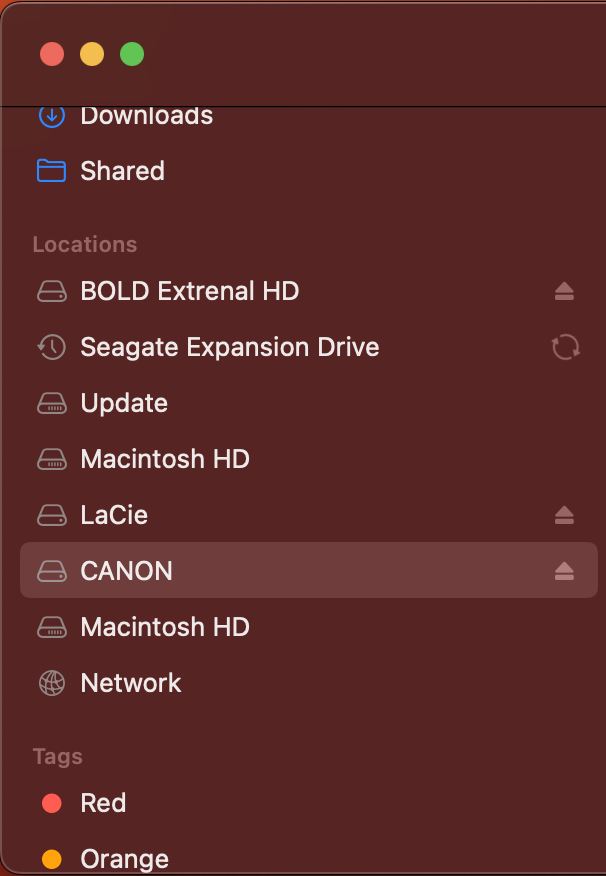
\includegraphics[width=0.6\linewidth]{Canon} 

}

\caption{File location for SD card recordings}\label{fig:canon}
\end{figure}

\hypertarget{using-the-light-board}{%
\section{Using the light board}\label{using-the-light-board}}

\begin{itemize}
\item
  Prior to using the light board, make sure it is clean with no visible streaks as this will show up in the recording. There is spray and cloths by the black curtain which you can use to clean the light board.
\item
  If you are referring to points on a slide, you may find it useful to use control points to mark areas to point to when presenting.
\item
  The green string frame around the light board indicates areas where not to write when presenting. Be sure to write within this frame so it is picked up by the recording.
\end{itemize}

\begin{figure}

{\centering 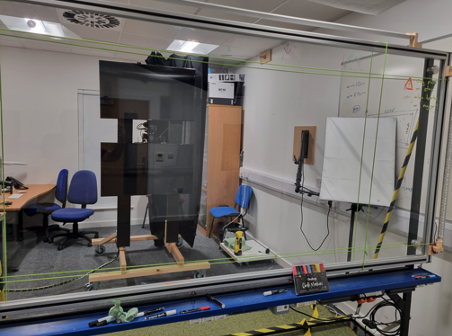
\includegraphics[width=0.6\linewidth]{Lightboard} 

}

\caption{Light board recording area (within green frame)}\label{fig:lightboard}
\end{figure}

\begin{itemize}
\tightlist
\item
  There are pens to use specifically for the light board. These sometimes need to be primed so press back and forth on the tip for a minute to ensure the ink has filled the tip. If all of the pens run dry, let the ODL management team know so more can be ordered.
\end{itemize}

\begin{figure}

{\centering 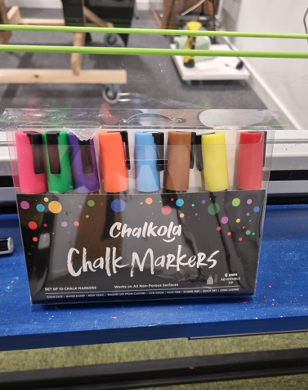
\includegraphics[width=0.6\linewidth]{Pens} 

}

\caption{Markers to be used for light board}\label{fig:pens}
\end{figure}

\hypertarget{storing-files-on-the-mac}{%
\section{Storing files on the Mac}\label{storing-files-on-the-mac}}

\begin{itemize}
\tightlist
\item
  Once you have completed your recordings and any editing, save the files you wish to keep on the LaCie drive shown below. Create a folder to store your work on the drive and remove any files from the BOLD account once completed.
\end{itemize}

\begin{figure}

{\centering 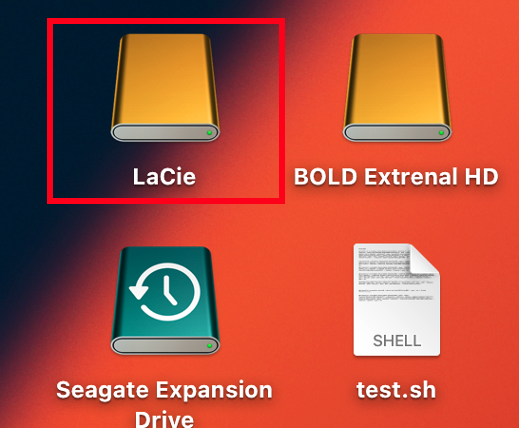
\includegraphics[width=0.4\linewidth]{Lacie} 

}

\caption{LaCie drive for file storage}\label{fig:lacie}
\end{figure}

\hypertarget{finishing-up}{%
\section{Finishing up}\label{finishing-up}}

\begin{itemize}
\item
  Once you are finished, check the battery level on the microphones. If these are low, please change these with new batteries and charge those removed.
\item
  Shut down the Mac and place the keyboard/mouse on charge with the charging cable underneath the Mac.
\item
  Put main lights on in room and turn off all other lights including lightboard.
\item
  Ensure camera is switched off.
\item
  Turn off HDMI matrix.
\item
  Make sure all monitors are switched off.
\item
  Turn off LED no entry sign.
\end{itemize}

\hypertarget{using-final-cut-for-video-editing}{%
\chapter{Using Final Cut for video editing}\label{using-final-cut-for-video-editing}}

When you have finished recording your material, you will have to edit and piece together any recordings and screen captures you have created. This can be done using the video editing software Final Cut which can be found on the Mac.

This section will focus on how to edit a video combining both a camera recording and a screen capture. If you are editing only a camera recording, some of the following steps may be omitted.

\hypertarget{prior-to-opening-final-cut}{%
\section{Prior to opening Final Cut}\label{prior-to-opening-final-cut}}

Ensure you have copied across the recording from the camera which is saved in the SD card and uploaded this to the Mac. Locate your screen capture recording if you have this.

\hypertarget{setting-up-final-cut}{%
\section{Setting up Final Cut}\label{setting-up-final-cut}}

\begin{itemize}
\tightlist
\item
  Open Final Cut. You can find Final Cut in the dock as shown below.
\end{itemize}

\begin{figure}

{\centering 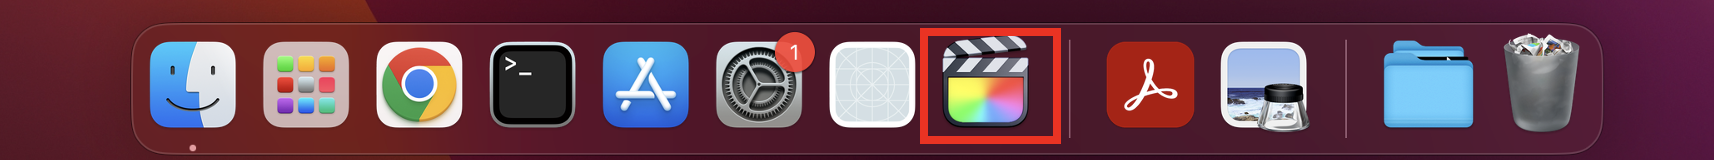
\includegraphics[width=1\linewidth]{FinalCutTab} 

}

\caption{Final Cut icon}\label{fig:fcdock}
\end{figure}

\begin{itemize}
\tightlist
\item
  When you first open Final Cut, you should see an empty display like the one below. If a library is already open, go to File \textgreater{} Close Library.
\end{itemize}

\begin{figure}

{\centering 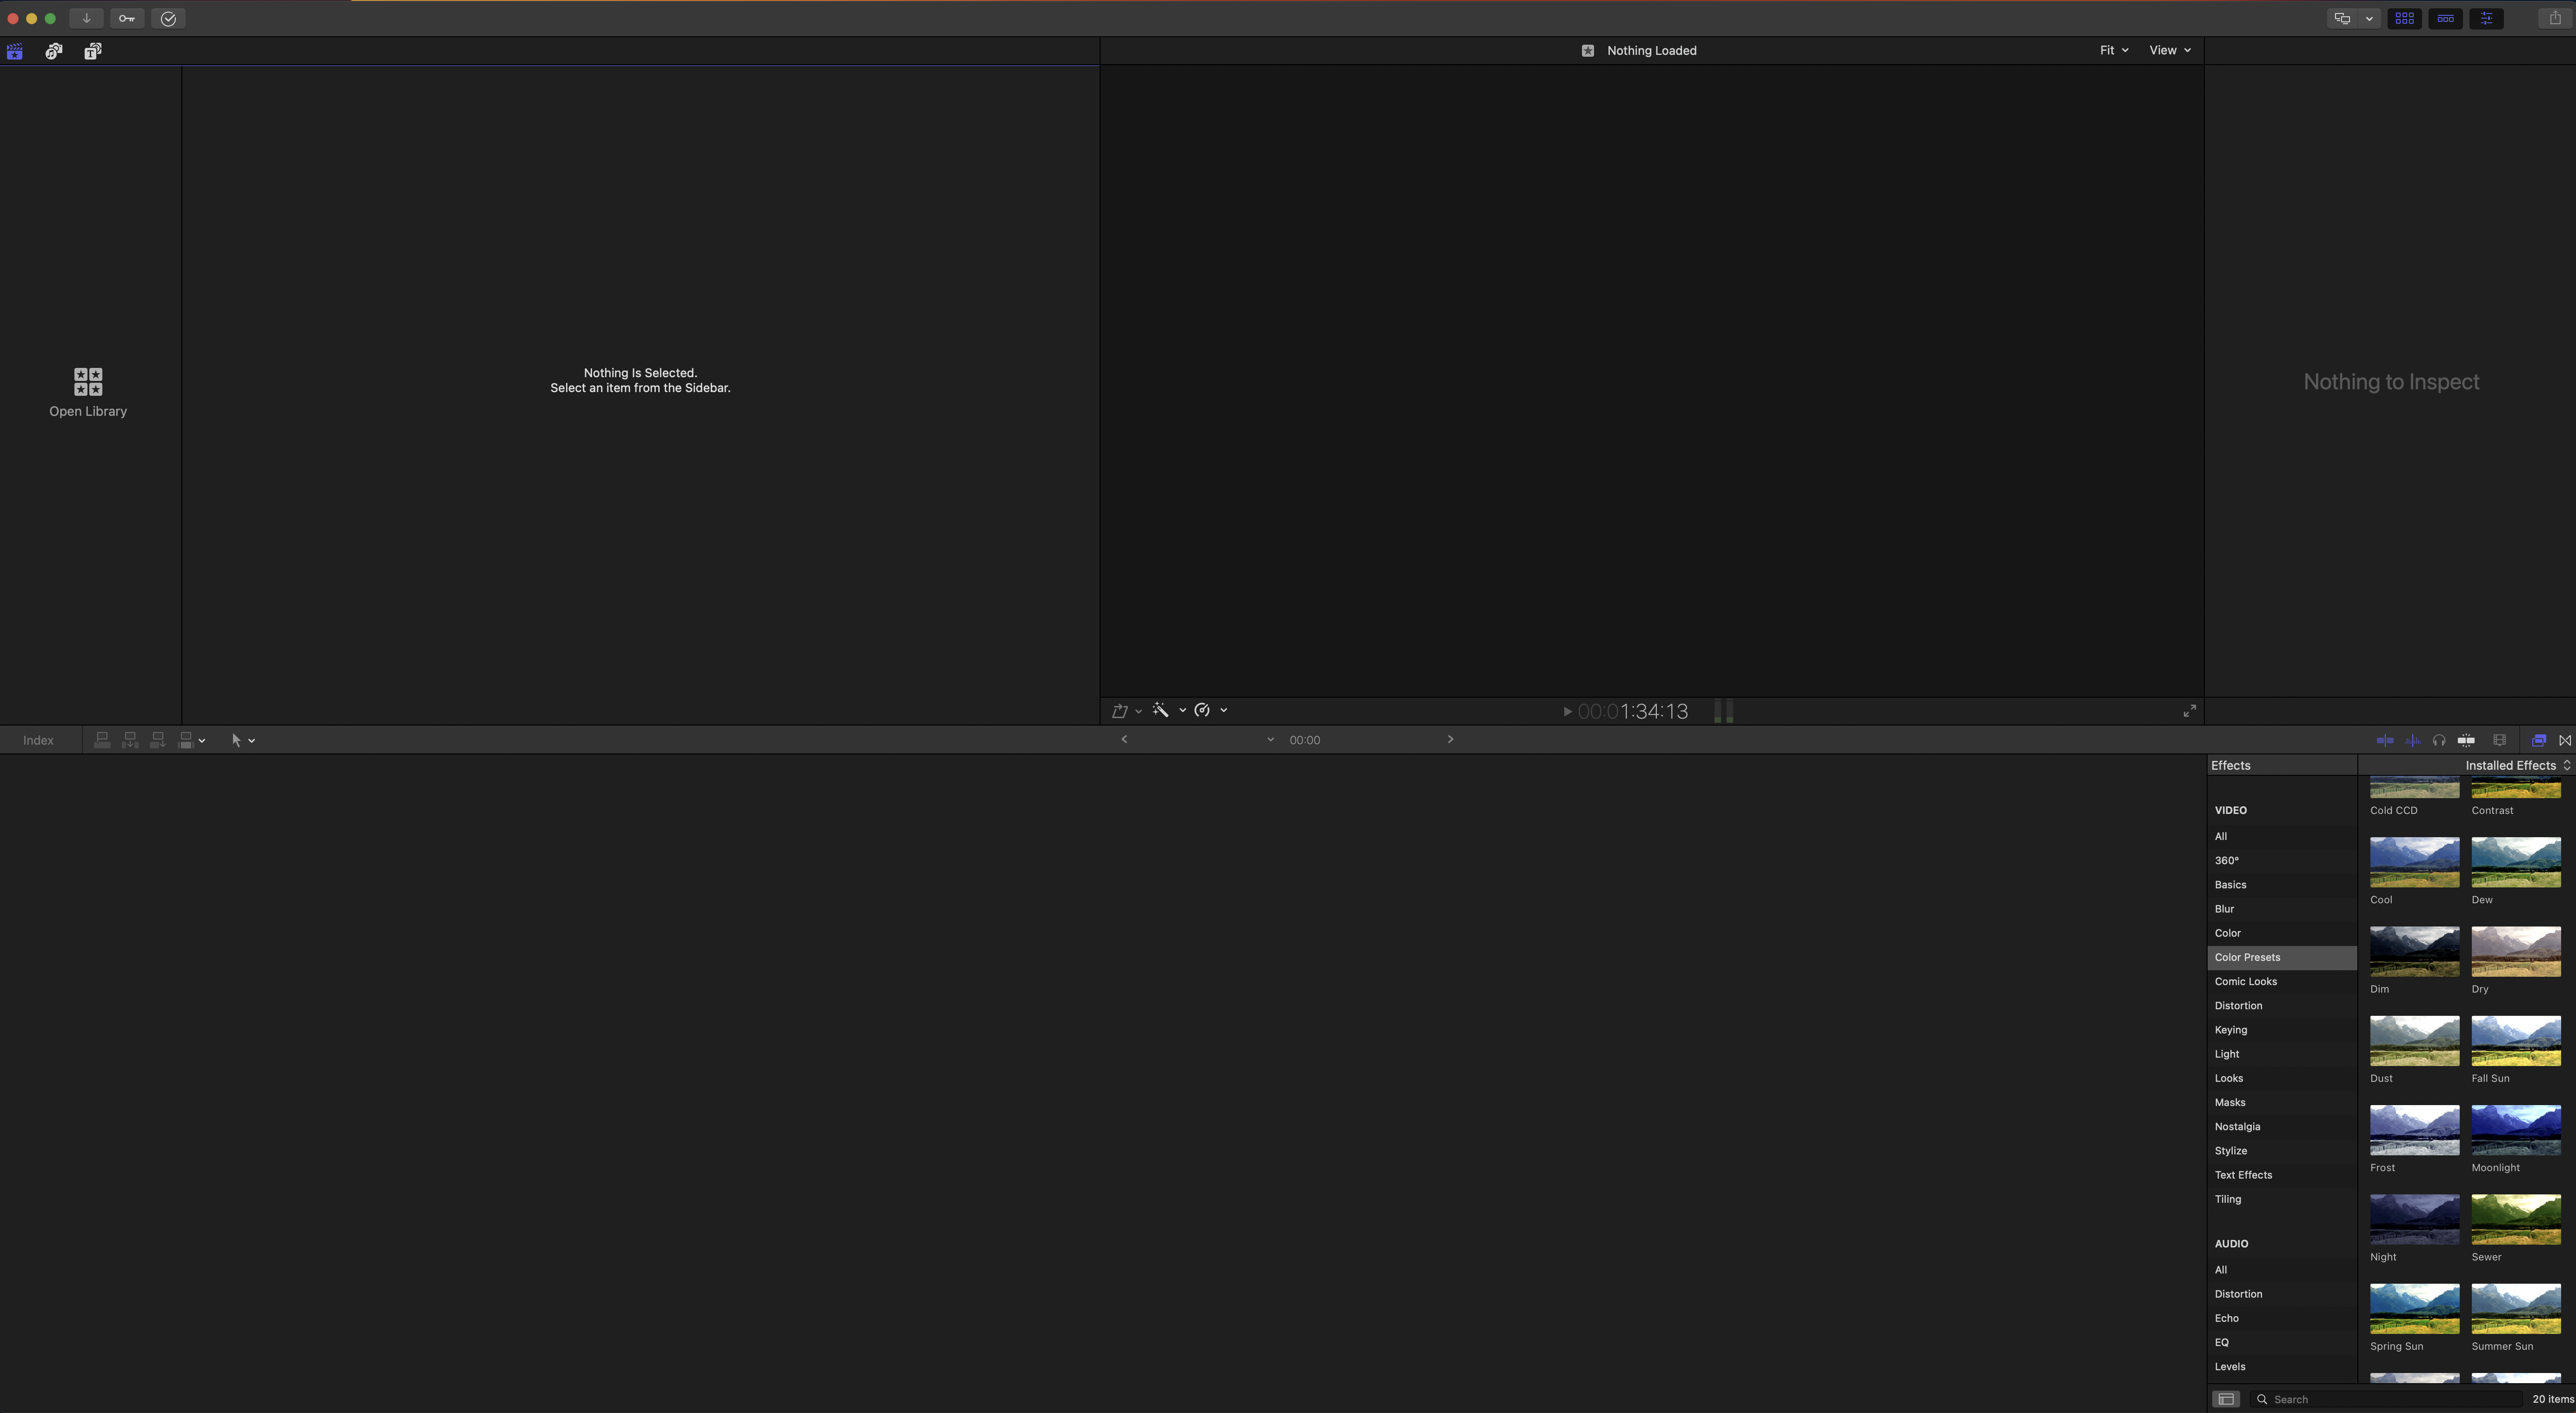
\includegraphics[width=1\linewidth]{FinalCutDisplay} 

}

\caption{Final Cut initial display}\label{fig:fcmenu}
\end{figure}

\begin{itemize}
\item
  Create a new library using File \textgreater{} New \textgreater{} Library. Name your library something meaningful such as ``Course x'', ``Week 1 -- Course y''. Your library will consist of multiple events.
\item
  Once your library has been created, an event will be automatically created with the current date, which you can see in the top left panel. You can rename this event by double clicking on the name or create a new event by right clicking on this area and selecting New Event.
\end{itemize}

\begin{figure}

{\centering 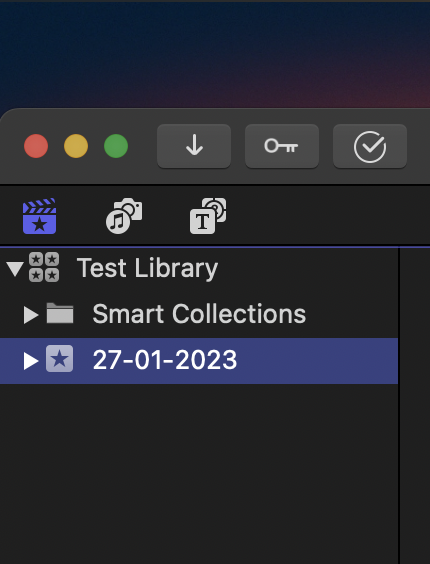
\includegraphics[width=0.5\linewidth]{Event} 

}

\caption{New event created with library}\label{fig:event}
\end{figure}

\begin{itemize}
\tightlist
\item
  To begin editing your video, you will need to create a new project within your event. You can do this by right clicking on your event and selecting New Project. Name your project and select OK.
\end{itemize}

\begin{figure}

{\centering 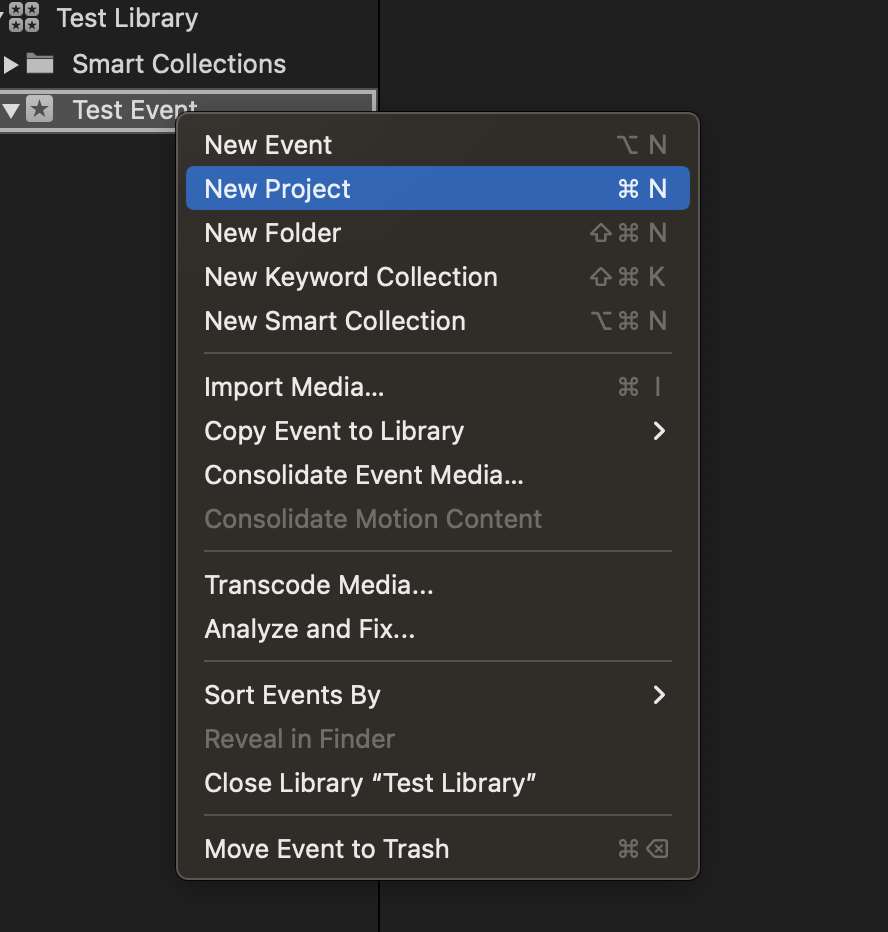
\includegraphics[width=0.5\linewidth]{Project} 

}

\caption{New event created with library}\label{fig:project}
\end{figure}

\begin{itemize}
\tightlist
\item
  Once your project is open, you can either import both your screen recording and camera capture using the Import \textgreater{} Media option in Files or drag and drop both files into the recording pane in the bottom half of final cut.
\end{itemize}

\hypertarget{syncing-your-camera-recording-and-screen-capture}{%
\section{Syncing your camera recording and screen capture}\label{syncing-your-camera-recording-and-screen-capture}}

\textbf{NB - If you are only editing the camera recording, many of these steps can be omitted, and you will only have to change the scale and audio}

\begin{itemize}
\tightlist
\item
  Firstly, drag both the camera recording and screen capture onto the timeline on the bottom half of the Final Cut interface.
\end{itemize}

\begin{figure}

{\centering 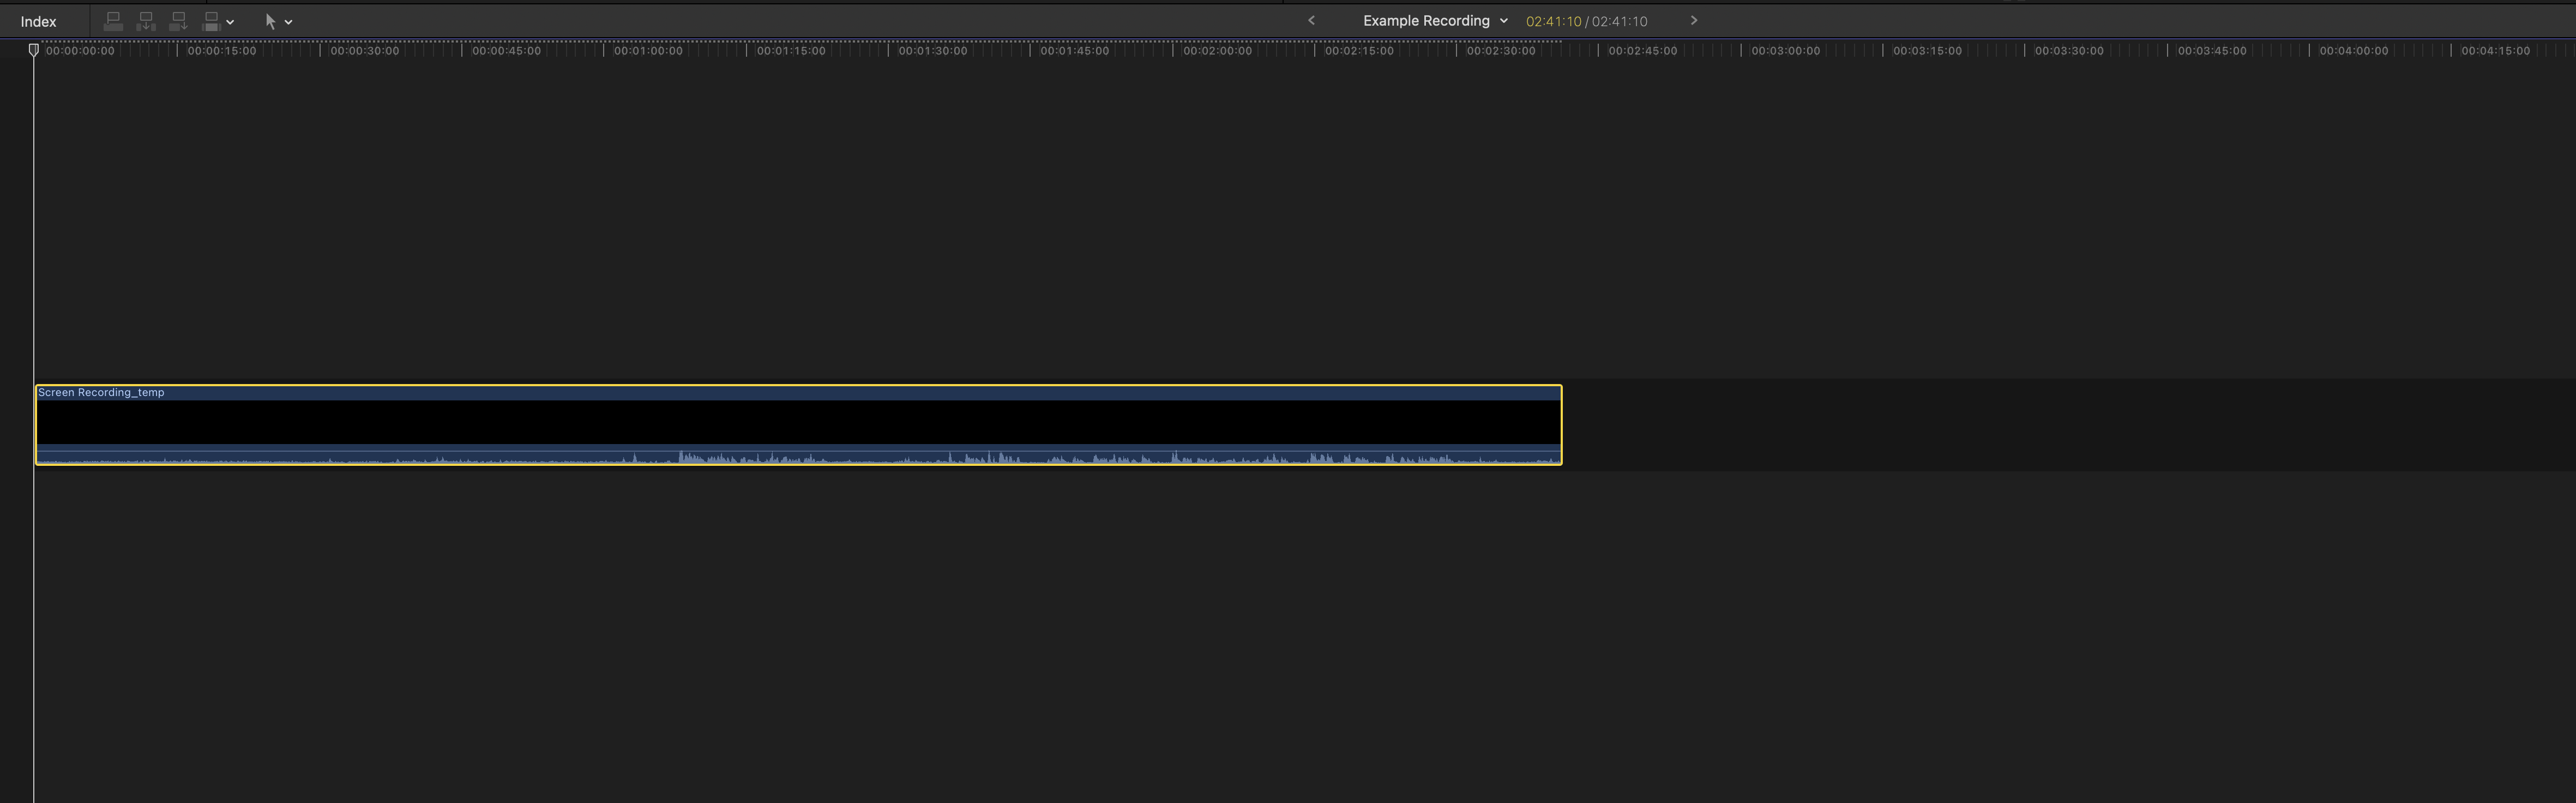
\includegraphics[width=1\linewidth]{FinalCutTimeline} 

}

\caption{Final Cut timeline}\label{fig:timeline}
\end{figure}

\begin{itemize}
\item
  Ensure that the screen capture video is at the top of the display and the camera recording is at the bottom on the timeline.
\item
  Firstly, you will need to combine the screen capture and camera recording together. This can be done by heading to the top left corner of the Final Cut interface, selecting the Film icon, then selecting All in Blend Mode.
\end{itemize}

\begin{figure}

{\centering 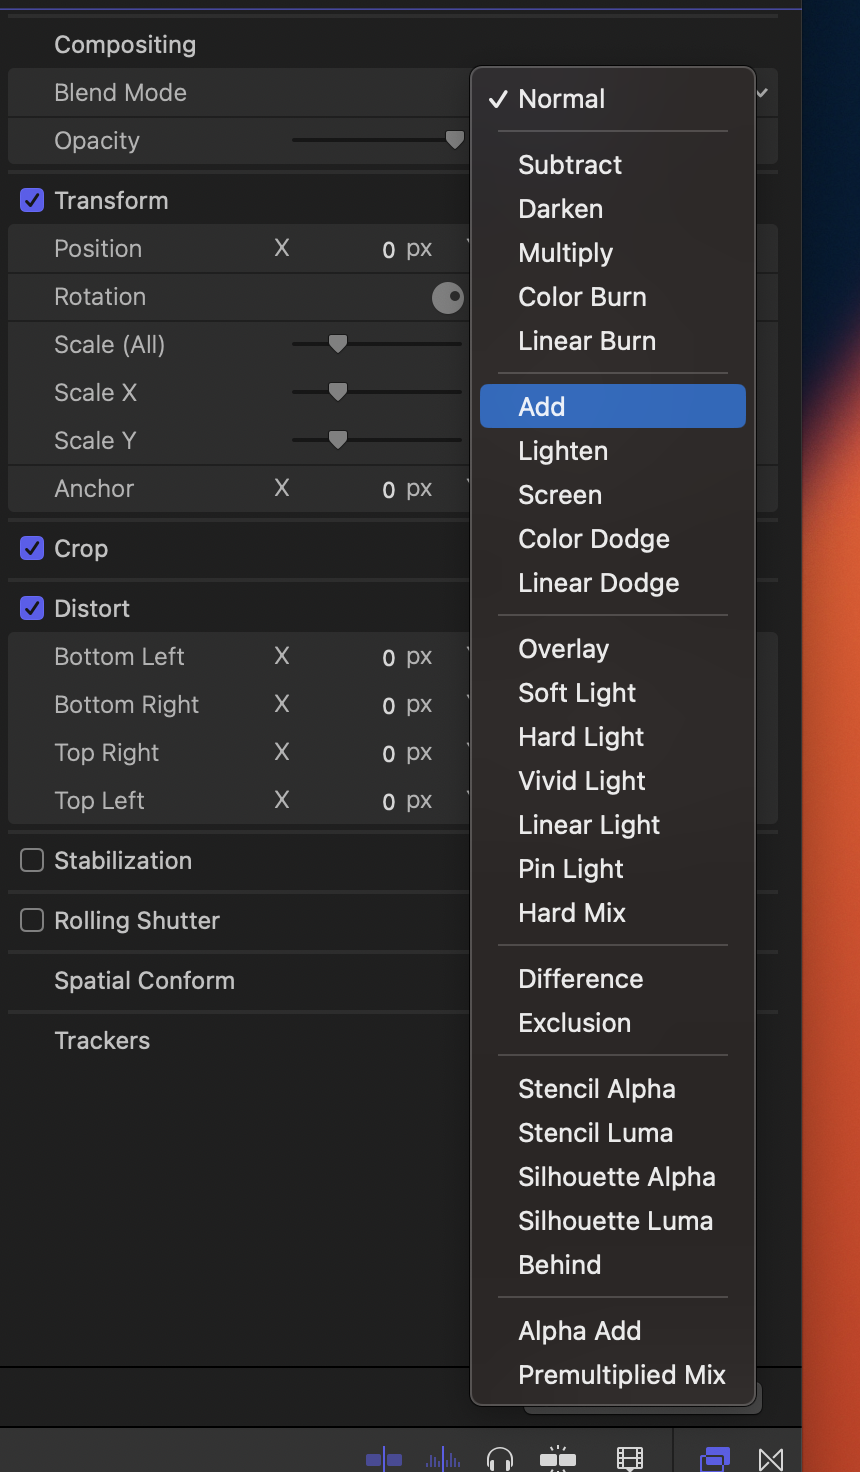
\includegraphics[width=0.6\linewidth]{BlendMode} 

}

\caption{Setting Blend Mode}\label{fig:blend}
\end{figure}

\begin{itemize}
\tightlist
\item
  Next, highlight the camera recording \textbf{only} on the timeline and change Scale x to -100\%. You can enter the numbers here by double clicking. This will flip the camera recording image.
\end{itemize}

\begin{figure}

{\centering 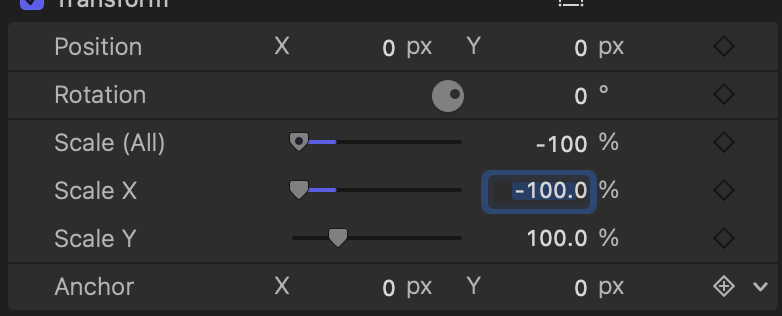
\includegraphics[width=1\linewidth]{ScaleX} 

}

\caption{Changing Scale x to flip video}\label{fig:scaleX}
\end{figure}

\begin{itemize}
\tightlist
\item
  With the camera recording still selected, now select the Audio menu in the top left corner (denoted by the speaker icon) and set the audio configuration to Dual Mono.
\end{itemize}

\begin{figure}

{\centering 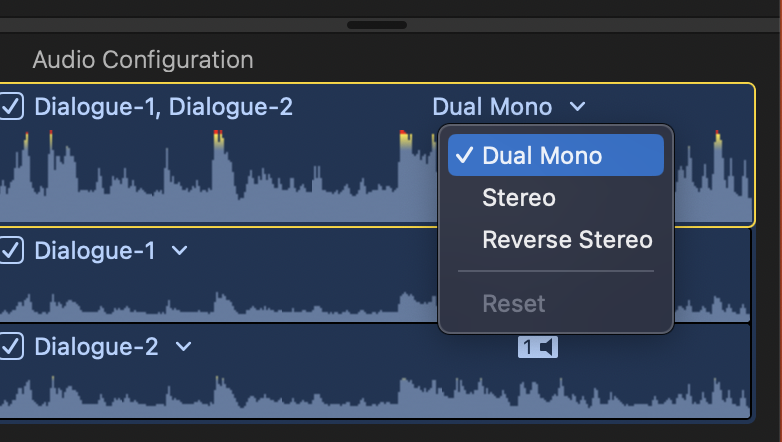
\includegraphics[width=1\linewidth]{Audio} 

}

\caption{Changing audio to Dual Mono}\label{fig:audio}
\end{figure}

\begin{itemize}
\item
  Next, match up your camera output and screen capture so they are in sync. You can do this by dragging the camera output file to align with the audio of the screen capture. You can use the soundwaves underneath the videos to help matching this. You can zoom in with the editor to make this easier using Command + (and Command - to zoom out again).
\item
  Finally, mute the sound on the screen capture video. You can do this by selecting the horizontal line on the video file in the timeline, above the sound file. Hold the left mouse button and drag down to mute.
\end{itemize}

\begin{figure}

{\centering 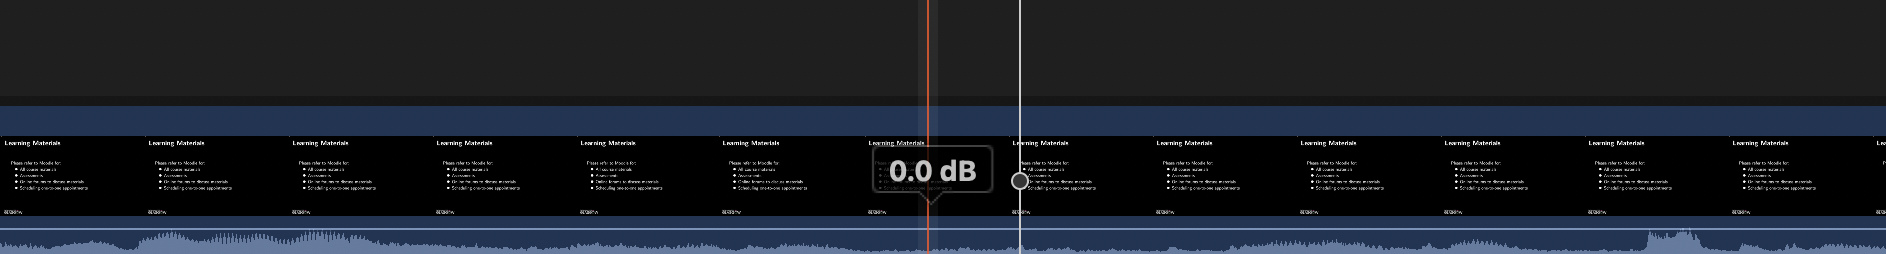
\includegraphics[width=1\linewidth]{Mute} 

}

\caption{Muting screen capture file}\label{fig:mute}
\end{figure}

\hypertarget{editing-the-video}{%
\section{Editing the video}\label{editing-the-video}}

\begin{itemize}
\item
  You may wish to add an introductory slide screen prior to your video beginning (like videos produced in ODL). The easiest way to do this is to take a screenshot of such a slide in full screen mode. You can do this by using Shift \textgreater{} Command \textgreater{} 3 which will save this to the desktop. Simply drag and drop the screen capture to your recording pane on Final Cut or use the Import command.
\item
  To transition between recordings, there is an option to include transitions. The most common type to use is ``Blurs'' and then ``Simple'', though do feel free to use any transitions you wish! Simply select and drag your chosen transition and place this between two video files for the transition to be included. You can alter the length of the transition by highlighting the edges of the transition window and dragging to increase/decrease the length. You can also add a transition using the hotkey shortcut Command + T
\end{itemize}

\begin{figure}

{\centering 
\includegraphics[width=0.6\linewidth]{Transition} 

}

\caption{Selecting transitions menu}\label{fig:transition}
\end{figure}

\begin{figure}

{\centering 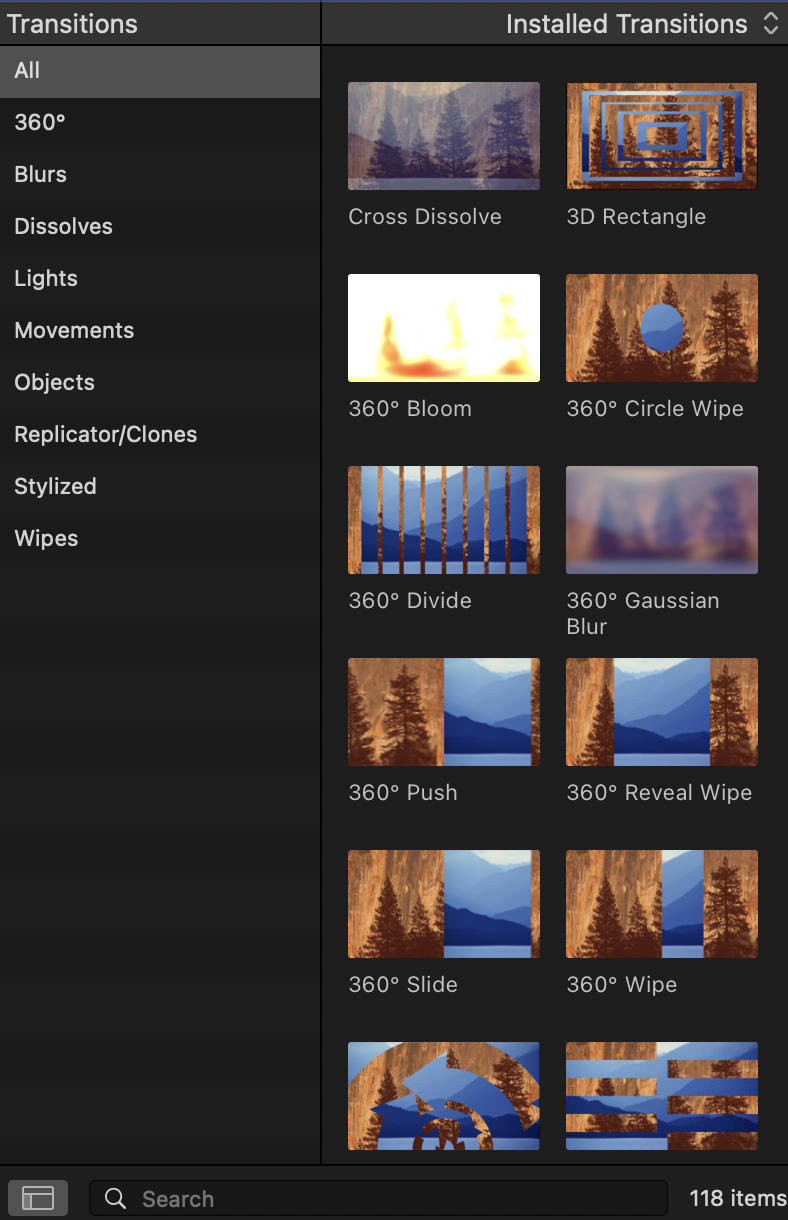
\includegraphics[width=1\linewidth]{TOptions} 

}

\caption{Transition options}\label{fig:toptions}
\end{figure}

\begin{figure}

{\centering 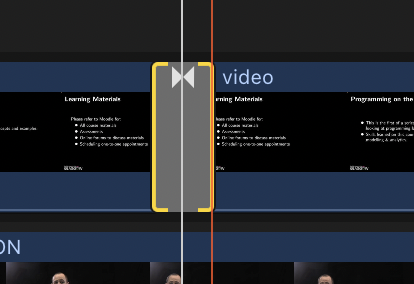
\includegraphics[width=1\linewidth]{TDrag} 

}

\caption{Controlling the time length of a transition}\label{fig:tdrag}
\end{figure}

\begin{itemize}
\tightlist
\item
  You can adjust the position and size of the speaker in your camera recording by highlighting the camera recording track and selecting the bottom left panel on the recording viewer. This will allow you to select the recording in the viewer and change the size and scale much like an image in Word. You can also crop, distort and transform using the other options.
\end{itemize}

\begin{figure}

{\centering 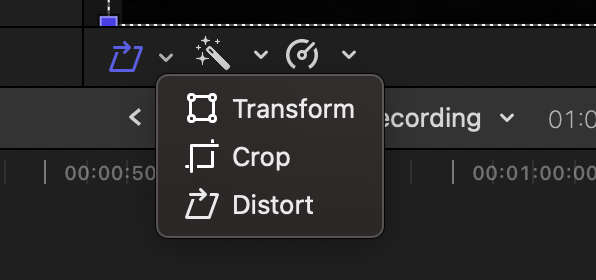
\includegraphics[width=1\linewidth]{Transform} 

}

\caption{Transforming camera image size and position options}\label{fig:transform}
\end{figure}

\begin{itemize}
\tightlist
\item
  You can also mask out any potential issues in your recording, for example smudges on the light board, heavily lit areas or exposed furniture by using the Effects panel. From here, you can select Masks and select from the options by double clicking your choice. This will open a new pane on the top right for you to alter the Mask to your liking.
\end{itemize}

\begin{figure}

{\centering 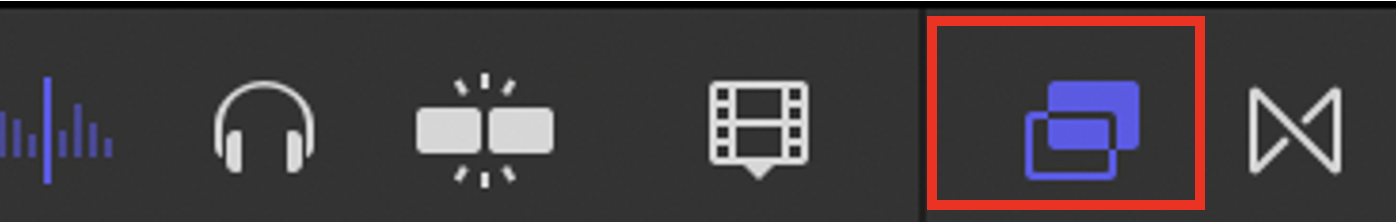
\includegraphics[width=0.6\linewidth]{Effects} 

}

\caption{Selecting effects option}\label{fig:effects}
\end{figure}

\begin{figure}

{\centering 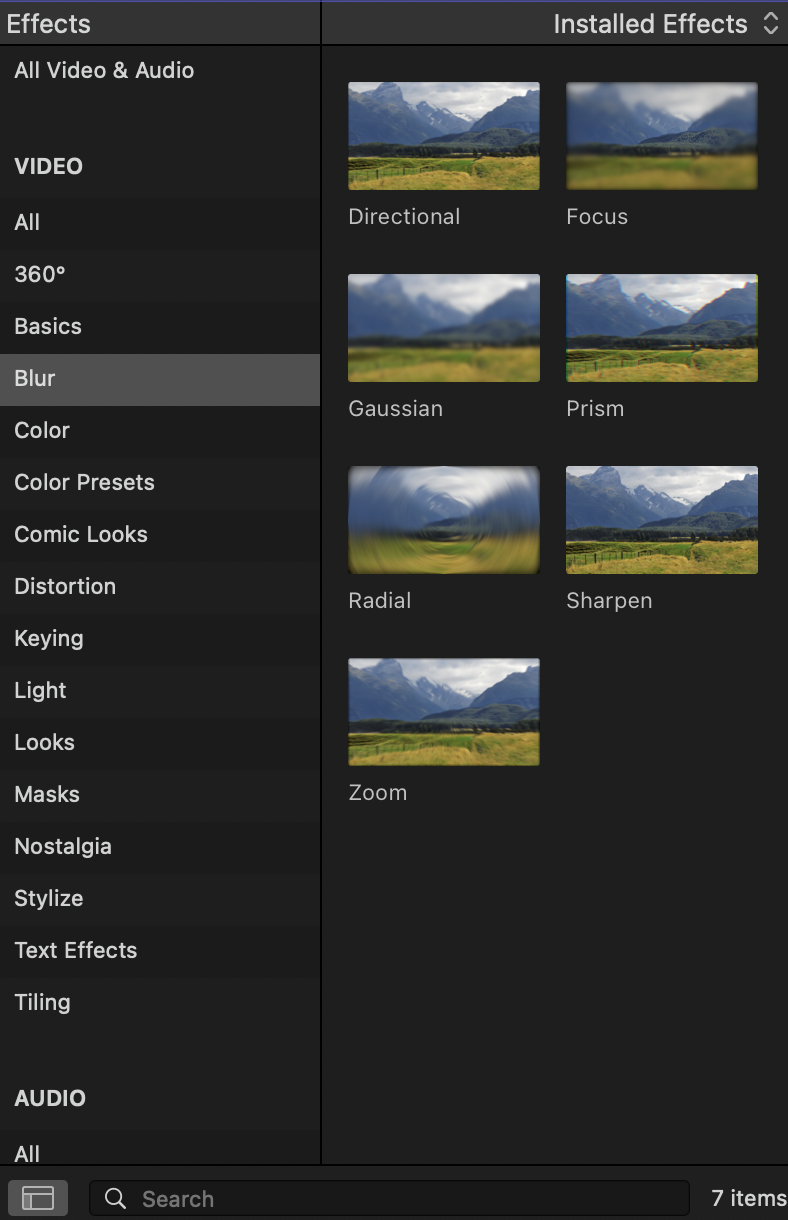
\includegraphics[width=1\linewidth]{EOptions} 

}

\caption{Effects options for masking}\label{fig:eoptions}
\end{figure}

\begin{figure}

{\centering 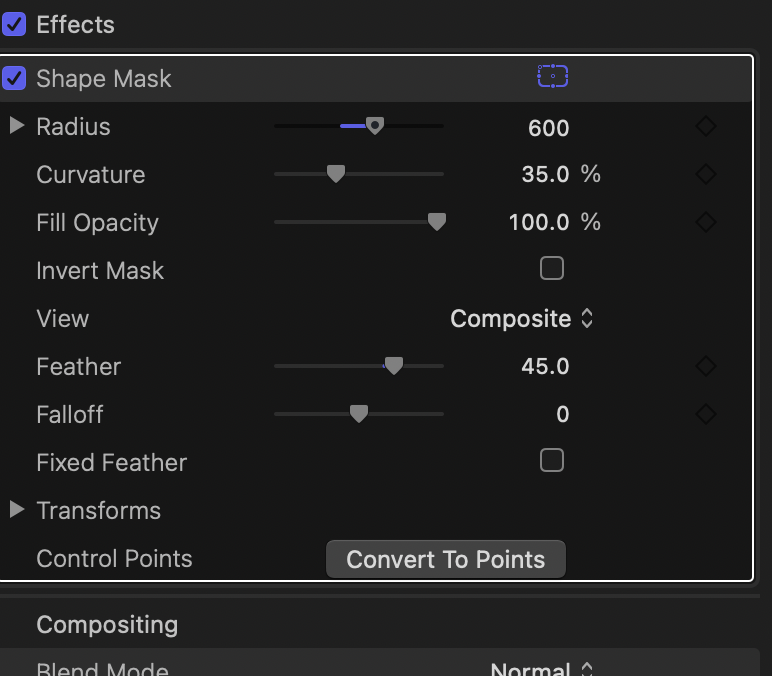
\includegraphics[width=1\linewidth]{Emenu} 

}

\caption{Menu to control aspects of masking}\label{fig:emenu}
\end{figure}

\hypertarget{hot-keys}{%
\section{Hot Keys}\label{hot-keys}}

When editing your video, you may find the following hot key options useful when editing on the timeline. You can select all of these options in the standard menu though if you wish.

\begin{itemize}
\item
  Command +, Command - - Zoom in/out through time in timeline
\item
  Command Z - Undo previous command
\item
  Command T - Add transition
\item
  Control D - Controls the duration of the current selection (good for editing transitions and slide captures)
\item
  H - Hand tool (this is used to scroll through timeline)
\item
  P - Position tool (this is used to place clips precisely)
\item
  A - Arrow tool for selection
\item
  B - Blade tool. This is used to crop sections of a recording. Select section of a recording where you wish to cut. You can then remove this section by pressing delete.
\end{itemize}

\hypertarget{saving-your-recording.}{%
\section{Saving your recording.}\label{saving-your-recording.}}

\begin{itemize}
\item
  Once you have finished editing your recording, you can save your final version by going to File \textgreater{} Share \textgreater{} Export file.
\item
  A menu will appear like the one shown before. You can change the video codec here to the file output you desire. The most common format to use is H264.
\end{itemize}

\begin{figure}

{\centering 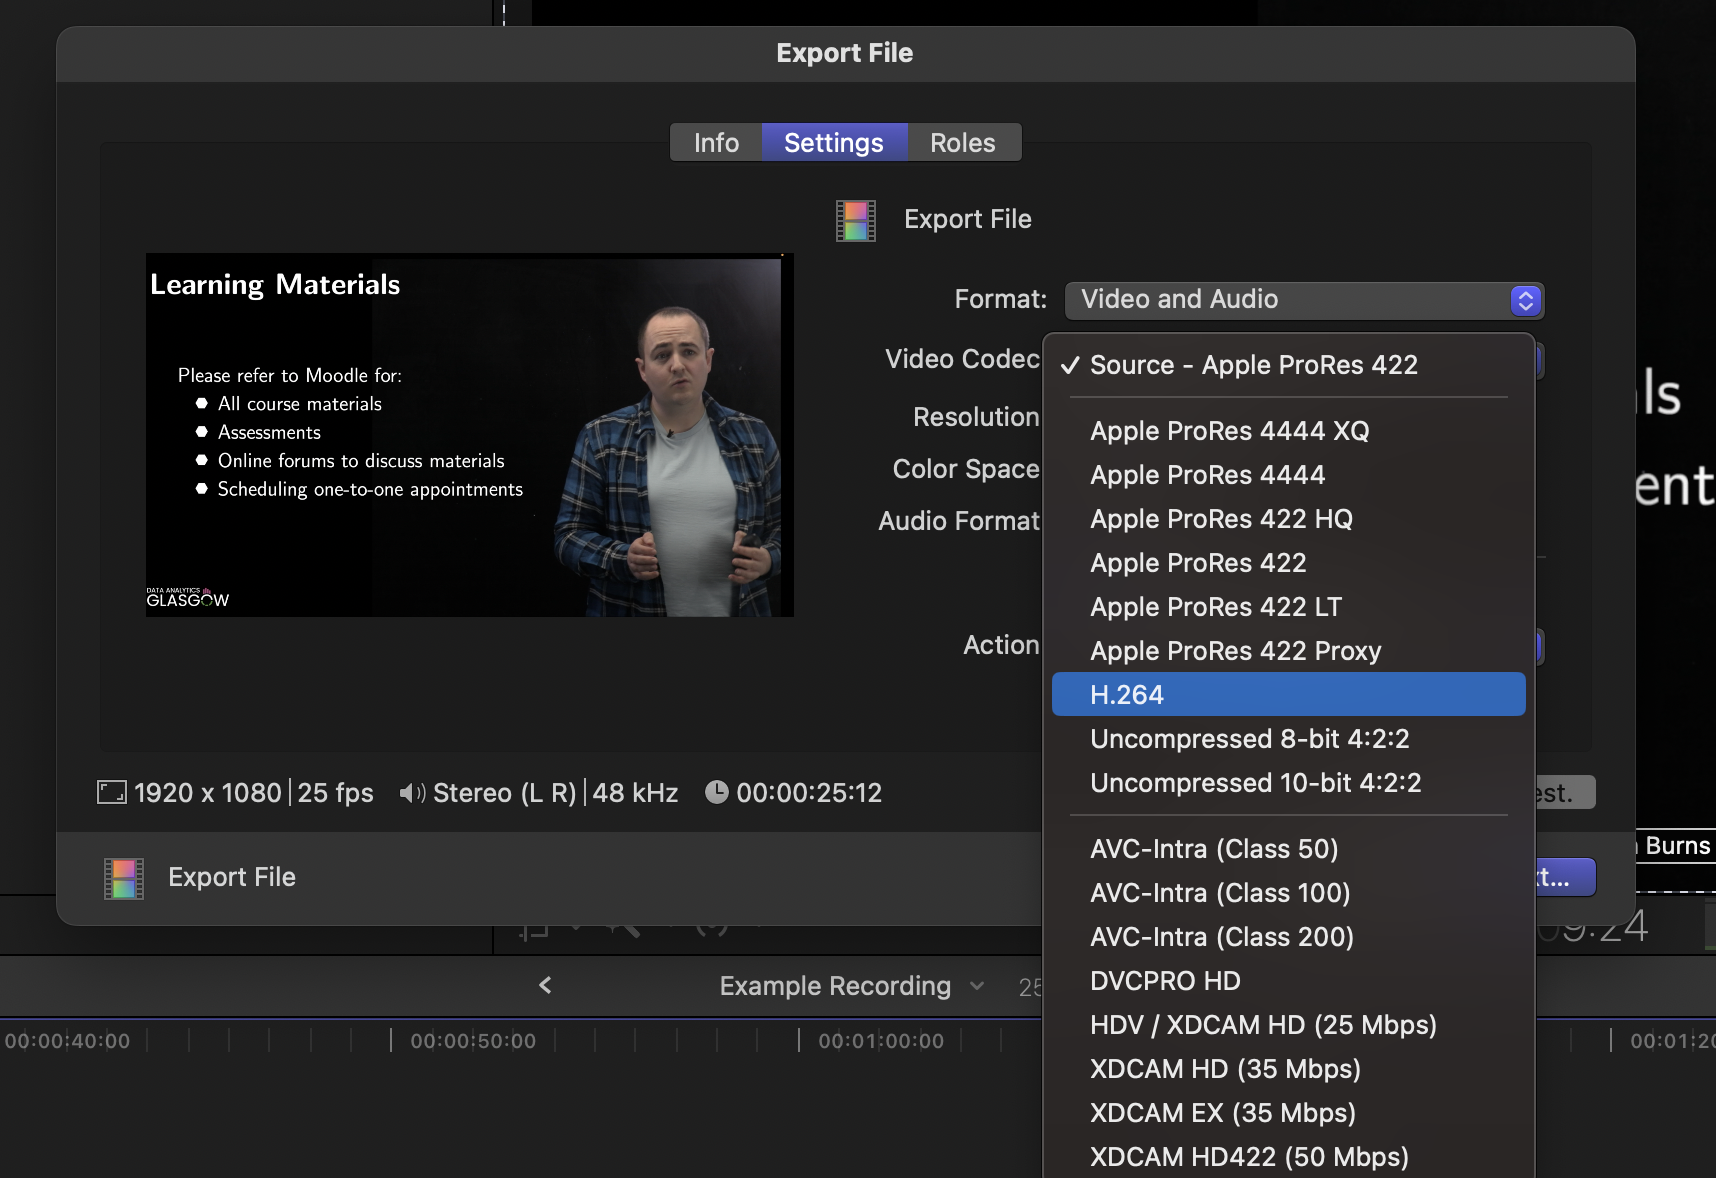
\includegraphics[width=1\linewidth]{Saving} 

}

\caption{Exporting your video and setting format}\label{fig:saving}
\end{figure}

\begin{itemize}
\tightlist
\item
  \textbf{ODL only} You can export your video to YouTube to the ODL channel for sharing by selecting File \textgreater{} Share \textgreater{} YouTube. Put settings to HD1080p with privacy unlisted. Final cut will then export your video to the ODL YouTube channel UofG\_AnalyticsMSc. Once this is completed, a dialogue box will appear at the top right of Final Cut.
\end{itemize}

\hypertarget{using-the-wacom-for-screen-capture}{%
\chapter{Using the Wacom for screen capture}\label{using-the-wacom-for-screen-capture}}

For recording screen captures of video tutorials or coding examples, the Wacom tablet located in the middle of the room on the left wall is the best device to use.

The Wacom is a large tablet device which can be used for written tutorials, similarly to an iPad. The Wacom is connected to the nearby Windows machine which should be switched on. You can log in using your GUID.

\hypertarget{setting-up-screen-capture}{%
\section{Setting up screen capture}\label{setting-up-screen-capture}}

\begin{itemize}
\item
  To capture your active screen on the Wacom, you can use OBS Studio which is located on the desktop.
\item
  Once OBS Studio is open, select the Wacom display from the display options to capture this screen (you can drag any additional open windows over to the monitor on the Windows machine). For the video settings, set the video resolution to 1280 x 1024 for base and output.
\item
  For the file type, save this as a .flv file. This will be converted on the Mac.
\item
  Set your file path to the desired location (Videos is often the default).
\item
  For the display capture, to ensure that the Wacom is available, you may need to add in the source. This can be done by selecting Sources and ``Add display capture'', then adding Display 1.
\item
  Once set up, OBS Studio will start recording your screen once you press record. Ensure you have everything you wish to record active on the Wacom, and remove any additional windows. Mute any desktop sounds.
\item
  Sound recording can be performed using either the headset or the microphone beside the Windows machine.
\end{itemize}

\hypertarget{using-smoothdraw-for-tutorial-videos}{%
\section{Using SmoothDraw for tutorial videos}\label{using-smoothdraw-for-tutorial-videos}}

\begin{itemize}
\item
  To produce written tutorial style videos, the programme SmoothDraw provides a nice interface to produce Khan Academy style tutorial videos. SmoothDraw can be found on the Desktop. If this is not visible, you can search for the application in the Start bar.
\item
  To ensure the full drawing palette is selected by the video, you will have to resize the palette. This can be done by selecting File \textgreater{} Resize. Untick both the width/height ratio options and set these to 1280 x 1024.
\item
  OBS Studio will show which area of the screen will be captured prior to recording, you can align SmoothDraw to fit within this window.
\item
  You may find it useful to change the palette colour to black (similarly to ODL tutorial videos) which can be changed in the ``Background'' layer option.
\item
  To set up writing, it is best to select the pen option for writing. You can set up shortcut keys for different colours, which can be useful for highlighting.
\item
  To show additional steps within a problem, you can use layers. On the left tab under Layers, you can ``select new layer'' which will create a new layer over the current palette to add new steps. Once these steps are shown, you can remove the layer by highlighting the new layer on the pane and pressing delete.
\end{itemize}

\hypertarget{editing-the-recording}{%
\section{Editing the recording}\label{editing-the-recording}}

\begin{itemize}
\item
  Once you have finished your recording, you can edit this in Final Cut using the Mac.
\item
  Transfer your recording to the Mac (either using a USB or transferring the file via OneDrive or a shared folder).
\item
  With your video recording, you will first have to change this to mp4 for editing. This can be performed using HandBrake which can transcode your video.
\item
  Open HandBrake (this can be found in the Dock). Once open, load your video file(s) by clicking on ``Source'' where you can select your videos for conversion.
\item
  Next, select your output format from the menu that appears. Select mp4.
\item
  You will have to ensure the picture resolution is correct. This can be checked by clicking the ``Picture Settings'' tab on the menu and ensuring this is set to 1280 x 1024).
\item
  The sound from your video may be quiet. You can check this prior to converting. If so, you can boost the sound by selecting the Audio tab on the menu and increasing the Gain (this can also be edited in Final Cut, so feel free to do this there).
\item
  Once all settings have been checked, convert the video by pressing the ``Start'' button, which will begin the conversion.
\item
  A pop-up will appear in the top right corner once this has been completed. You can then use your .mp4 video in Final Cut for editing.
\end{itemize}

  \bibliography{book.bib,packages.bib}

\end{document}
